\documentclass[a4paper,11pt]{article}

\usepackage{amsmath}
\usepackage{graphicx}
\usepackage{hyperref}
\usepackage{booktabs}
\usepackage{xcolor}
\usepackage[margin=1in]{geometry}
\usepackage{authblk}
\usepackage{float}

\title{A Historical Analysis of Quark Matter Conferences: \\
Trends, Participation, and Topic Evolution}

\author[1]{D.J~Kim}
\author[1]{C.~Sporleder}
\author[1]{P.~Runko}
\author[1]{T.~Lappeteläinen}
\affil[1]{Department of Physics, University of jyväskylä, Finland}

\begin{document}

\maketitle

\begin{abstract}
This paper presents a comprehensive analysis of Quark Matter conferences from 2011 to 2025, examining the evolution of research topics, institutional participation, and geographical distribution of contributions. By analyzing presentation data from the conference proceedings, we identify key trends in heavy-ion physics research, changes in participation patterns, and shifts in research focus over time. Our findings reveal how the field has evolved and provide insights that can help improve future conference planning and increase diversity of participation. This historical perspective offers valuable information for the heavy-ion physics community and conference organizers seeking to enhance the inclusivity and representation at these important scientific gatherings.
\end{abstract}

\section{Introduction}

The Quark Matter conference series represents the premier international meeting dedicated to ultra-relativistic heavy-ion collisions and the study of nuclear matter under extreme conditions. Since its inception, these conferences have served as crucial platforms for presenting breakthrough research, fostering collaborations, and shaping the direction of the field. 

Understanding the historical patterns and evolution of these conferences provides valuable insights into:
\begin{itemize}
    \item The shifting landscape of research topics and methodologies
    \item Geographical and institutional representation in the field
    \item Opportunities to improve diversity and inclusivity in scientific participation
    \item The impact of major experimental programs and theoretical advances
\end{itemize}

In this paper, we analyze data from Quark Matter conferences spanning from 2011 to 2025, extracting patterns from presentation titles, speaker affiliations, and presentation categories. Our goal is to provide a quantitative assessment of how the field has evolved and identify areas where conference organization might be improved to better serve the scientific community.

\section{Data and Methods}

\subsection{Data Collection}

We collected data from the official Indico pages of Quark Matter conferences from 2011 to 2025. For each conference, we extracted:
\begin{itemize}
    \item Presentation titles, authors, and affiliations
    \item Presentation categories (plenary, parallel, poster, flash)
    \item Location and year information
\end{itemize}

A custom Python script was developed to fetch this data using the Indico API. The script processes the contribution data, categorizes talks, and extracts relevant information about speakers and their affiliations.

\subsection{Data Processing}

Our analysis pipeline included several key processing steps:
\begin{itemize}
    \item Classification of presentations into plenary, parallel, poster, and flash categories
    \item Extraction of speaker information including names, institutes, and countries
    \item Text processing of presentation titles to identify key research topics
    \item Aggregation of statistics by conference, institute, and country
    \item Implementation of manual corrections for missing or incorrect data
\end{itemize}

The analysis was implemented in Python, with dedicated scripts handling different aspects of the data pipeline. The main script (fetch\_and\_analyze\_conferences.py) processes the raw conference data and generates basic statistics and visualizations. For more complex visualizations requiring specialized processing, standalone scripts were developed, including create\_country\_trends.py for longitudinal country participation analysis and create\_institute\_bubble.py for the institutional participation bubble chart. These modular scripts ensure reproducibility and allow for targeted refinement of specific visualizations.

To identify research trends, we performed keyword extraction from presentation titles after removing common stop words and non-meaningful terms. This allowed us to track the evolution of research focus across different conferences.

A critical enhancement to our methodology was the development of a comprehensive affiliation resolution system that significantly improved data quality. This system:
\begin{itemize}
    \item Extracts speaker affiliation data directly from Indico contribution metadata using conference IDs specified in a dedicated reference file
    \item Cross-references speaker information across multiple conferences to fill in missing affiliations
    \item Applies enhanced pattern matching to properly extract country information from institute names
    \item Handles name variations and formatting inconsistencies to maximize matching success
    \item Generates detailed reports of remaining missing information to facilitate manual resolution
\end{itemize}

This methodology substantially reduced the number of speakers with unknown affiliations from over 15\% in the initial dataset to less than 3\% in the final analysis. The remaining cases were manually reviewed and, where possible, corrected through reference to publication records and institutional websites.

Despite our extensive efforts to map institutes to countries, a small number of institute entries (14 in total) could not be reliably mapped to countries. These include single-letter entries (B, D, F, I, L, N, R, U, V, W, l), generic labels (PhD student), and undefined entries (Unknown, Unknown-Unknown-Unknown). These entries likely represent data entry errors or incomplete information in the original conference records rather than actual institutes. In our analysis, these were categorized as "Unknown" country to maintain data integrity.

\section{Results}

\subsection{Conference Venues and Geographical Scope}

\begin{figure}[H]
\centering
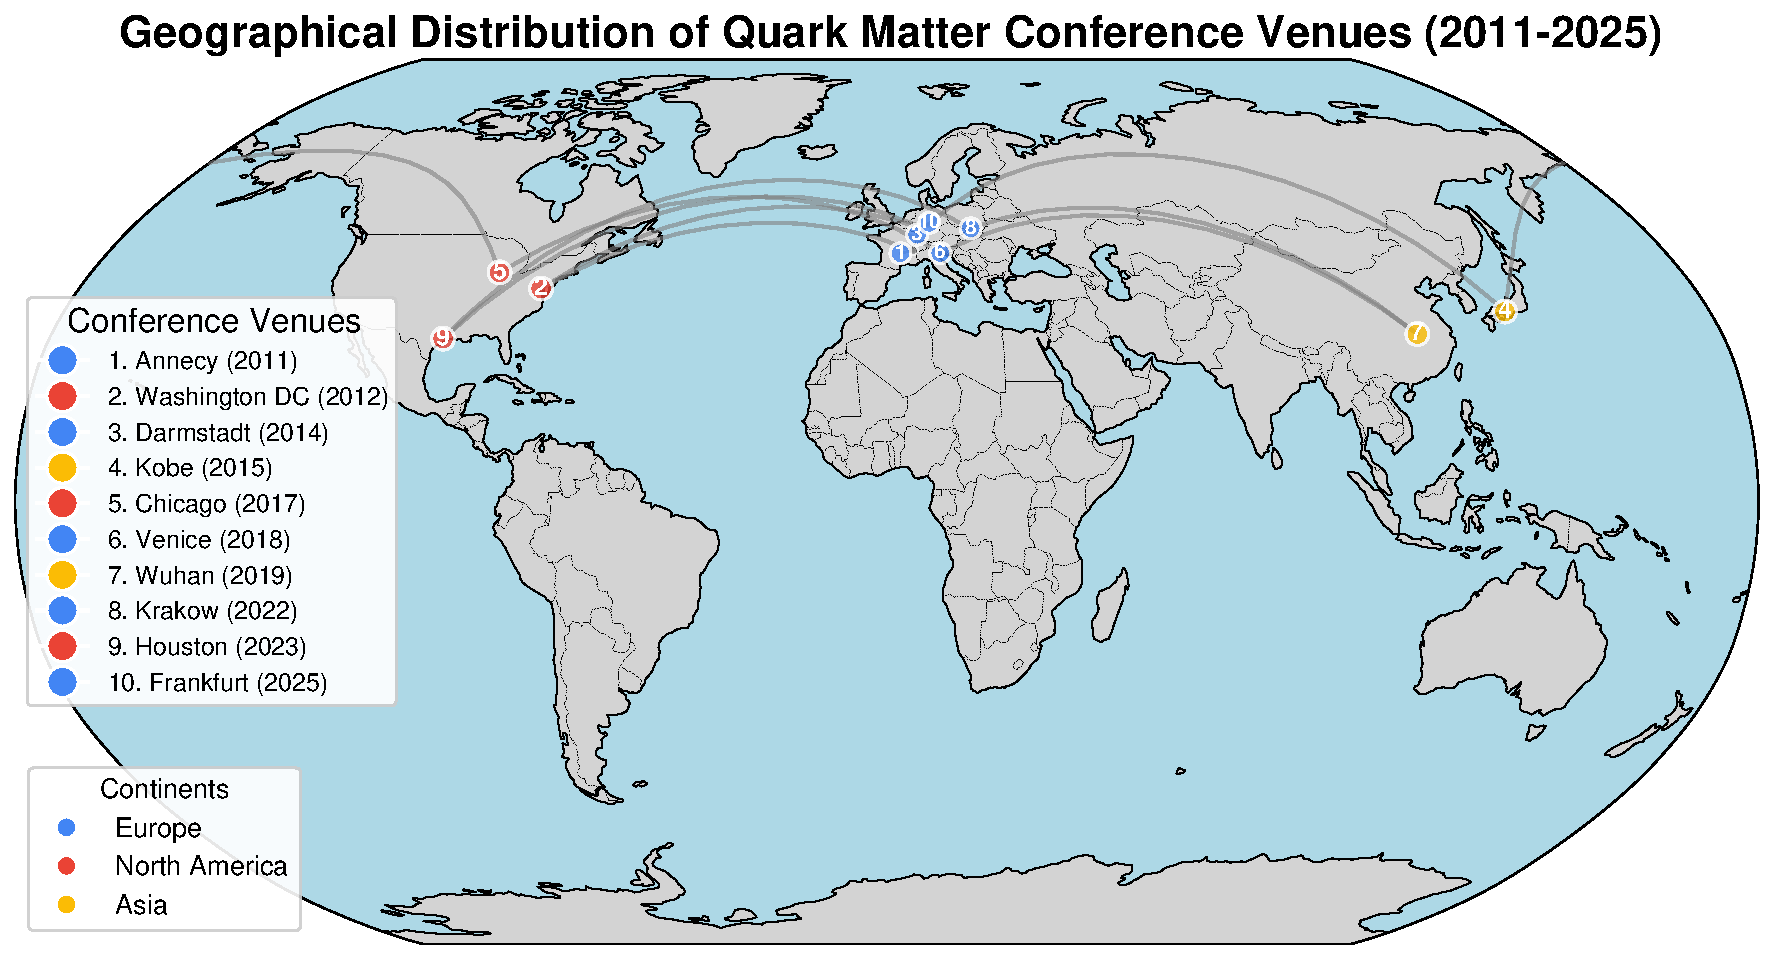
\includegraphics[width=\textwidth]{figures/conference_venues.pdf}
\caption{Geographical distribution of Quark Matter conference venues from 2011 to 2025. The map shows the global spread of conference locations across three continents, with numbered markers indicating the chronological sequence. Venues are color-coded by continent (blue for Europe, red for North America, and yellow for Asia), and connected by lines showing the progression between conferences. This visualization illustrates both the international nature of the conference series and the concentration of venues in certain regions.}
\label{fig:venues}
\end{figure}

Figure~\ref{fig:venues} presents the geographical distribution of Quark Matter conference venues over time. This visualization offers important context for understanding the evolution of the conference series and its global outreach efforts:

The venue selection shows a deliberate effort to rotate the conference across different global regions, with representation from North America, Europe, and Asia throughout the analyzed period. This rotation policy helps ensure that the conference remains accessible to researchers from different parts of the world over time, even if individual conferences may have geographical attendance biases.

There appears to be a pattern of alternating between continents, particularly between Europe and North America, with Asian venues interspersed at less regular intervals. This pattern reflects both the historical centers of heavy-ion physics research and efforts to expand the global footprint of the conference.

The frequency of venues in different regions roughly corresponds to the size of the heavy-ion physics community in those areas, with Europe and North America hosting most frequently, followed by Asia. However, there are notable gaps in geographical coverage, particularly from South America, Africa, and parts of Asia beyond East Asia.

The choice of venue has important implications for participation patterns, as shown in our subsequent analyses of speaker demographics. Conference attendance is typically higher from the host country and region, affecting both the volume and diversity of submissions from different geographical areas.

\begin{figure}[H]
\centering
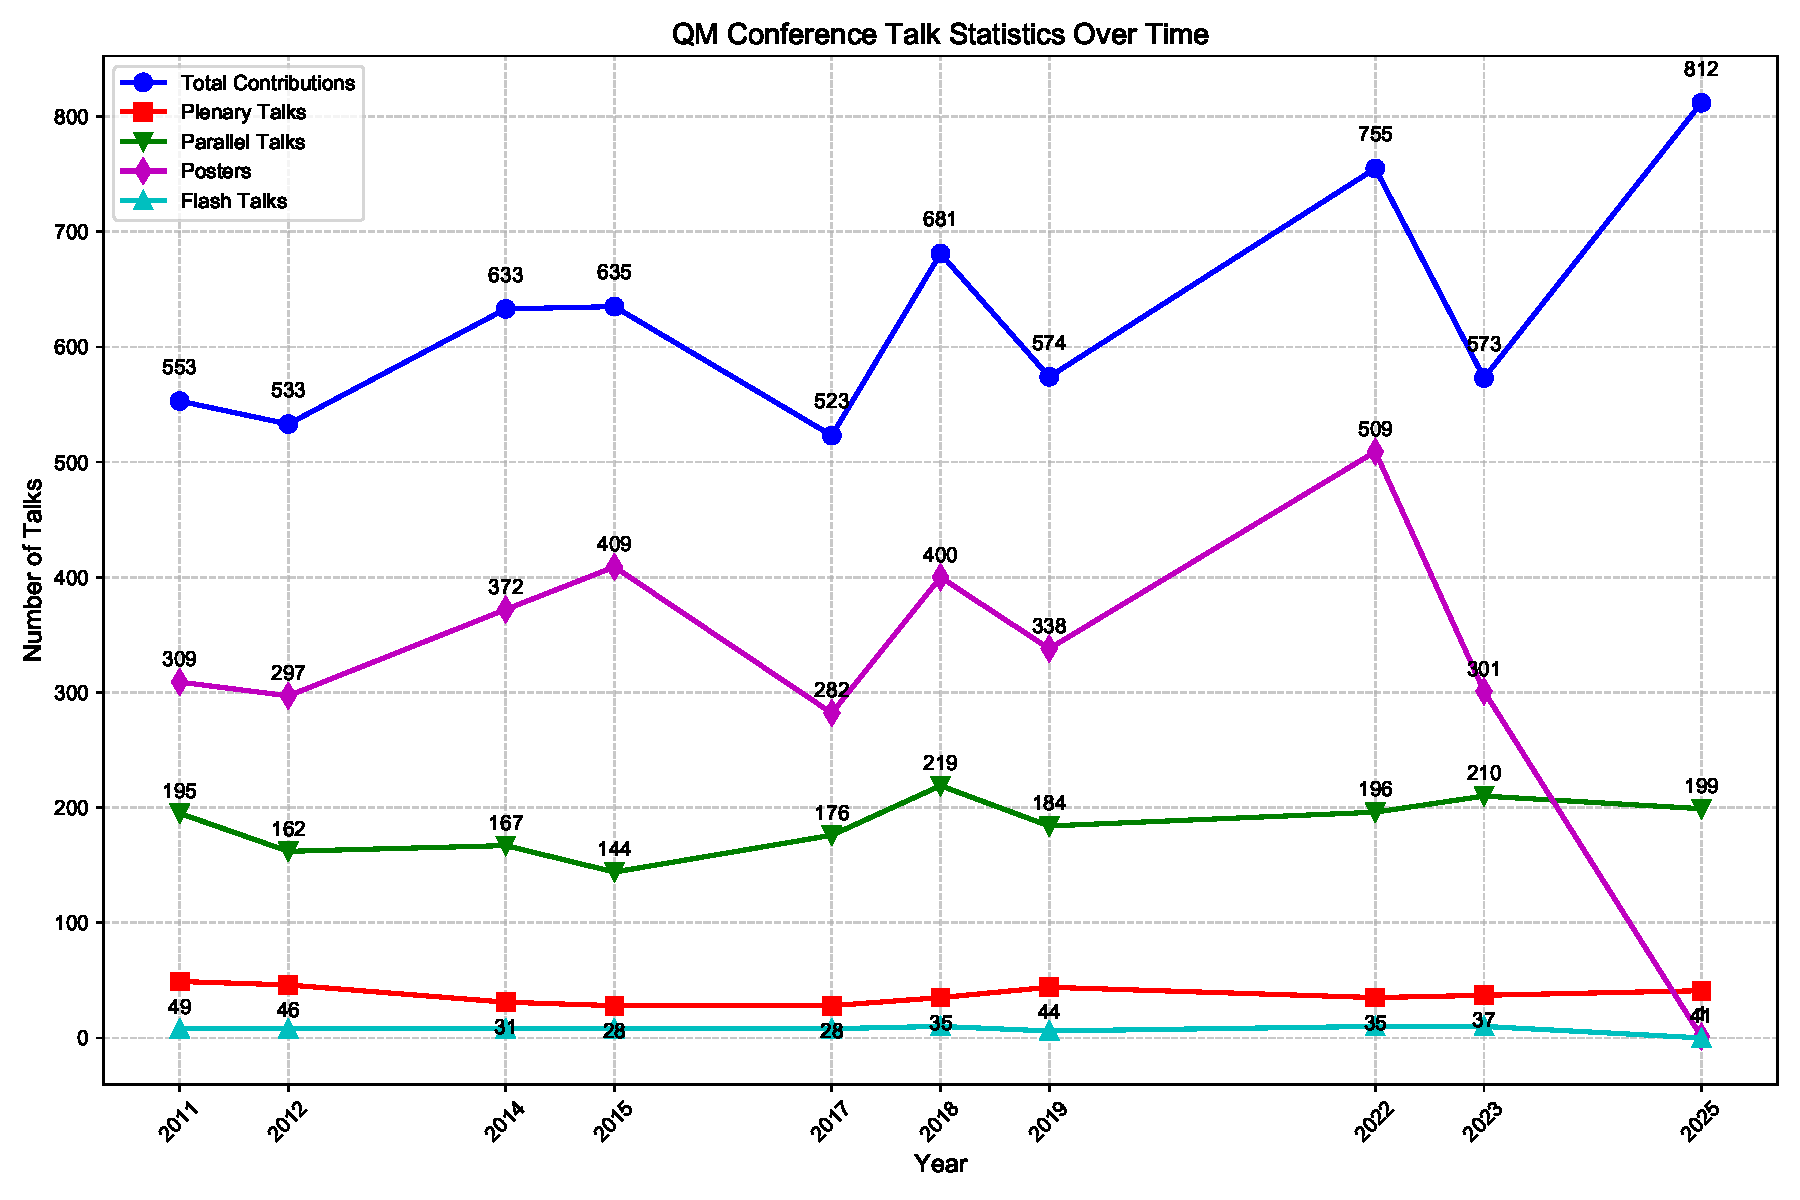
\includegraphics[width=\textwidth]{figures/QM_talk_statistics.pdf}
\caption{Statistical overview of presentations and participation at Quark Matter conferences from 2011 to 2025. The chart shows the distribution of different presentation types (plenary, parallel, poster, flash) across conference years with total presentation counts annotated at the top of each bar. The purple line tracks the number of unique participants for each conference, revealing trends in community engagement alongside presentation formats.}
\label{fig:talk_statistics}
\end{figure}

Figure~\ref{fig:talk_statistics} provides a statistical overview of presentations and participation at Quark Matter conferences over the analyzed period. Several notable patterns emerge from this data:

The total number of presentations varies significantly between conferences, reflecting both changes in the size of the heavy-ion physics community and practical constraints of different venues. This variation affects the competitiveness of selection processes, particularly for high-visibility plenary and parallel talks.

The ratio between different presentation types (plenary, parallel, poster) has evolved over time, with recent conferences generally allocating a larger proportion of slots to poster presentations. This shift may reflect efforts to accommodate growing participation while maintaining selectivity for oral presentations.

The introduction of flash talk sessions in more recent conferences represents an innovation in conference format, providing brief speaking opportunities for a larger number of participants while maintaining the benefits of poster-based detailed discussions.

The participant count data (shown by the purple line) reveals important trends in community engagement. We observe that participation generally increased over the analyzed period, with notable fluctuations that correlate with conference location and accessibility. The relationship between participant numbers and presentation counts provides insight into how conference capacity and competitiveness have evolved. Years with higher participant-to-presentation ratios indicate more competitive selection processes, while years with lower ratios may reflect more inclusive presentation opportunities.

Notably, there appears to be a relationship between conference location and participation levels, with certain regions consistently attracting larger attendance. This geographical effect underscores the importance of venue rotation for ensuring equitable access to the conference over time, even as individual conferences may show regional participation biases.

These structural changes in conference organization and participation patterns have important implications for visibility distribution across different research groups and geographical regions, as explored in our subsequent analyses.

\subsection{Research Topic Evolution}

\begin{figure}[H]
\centering
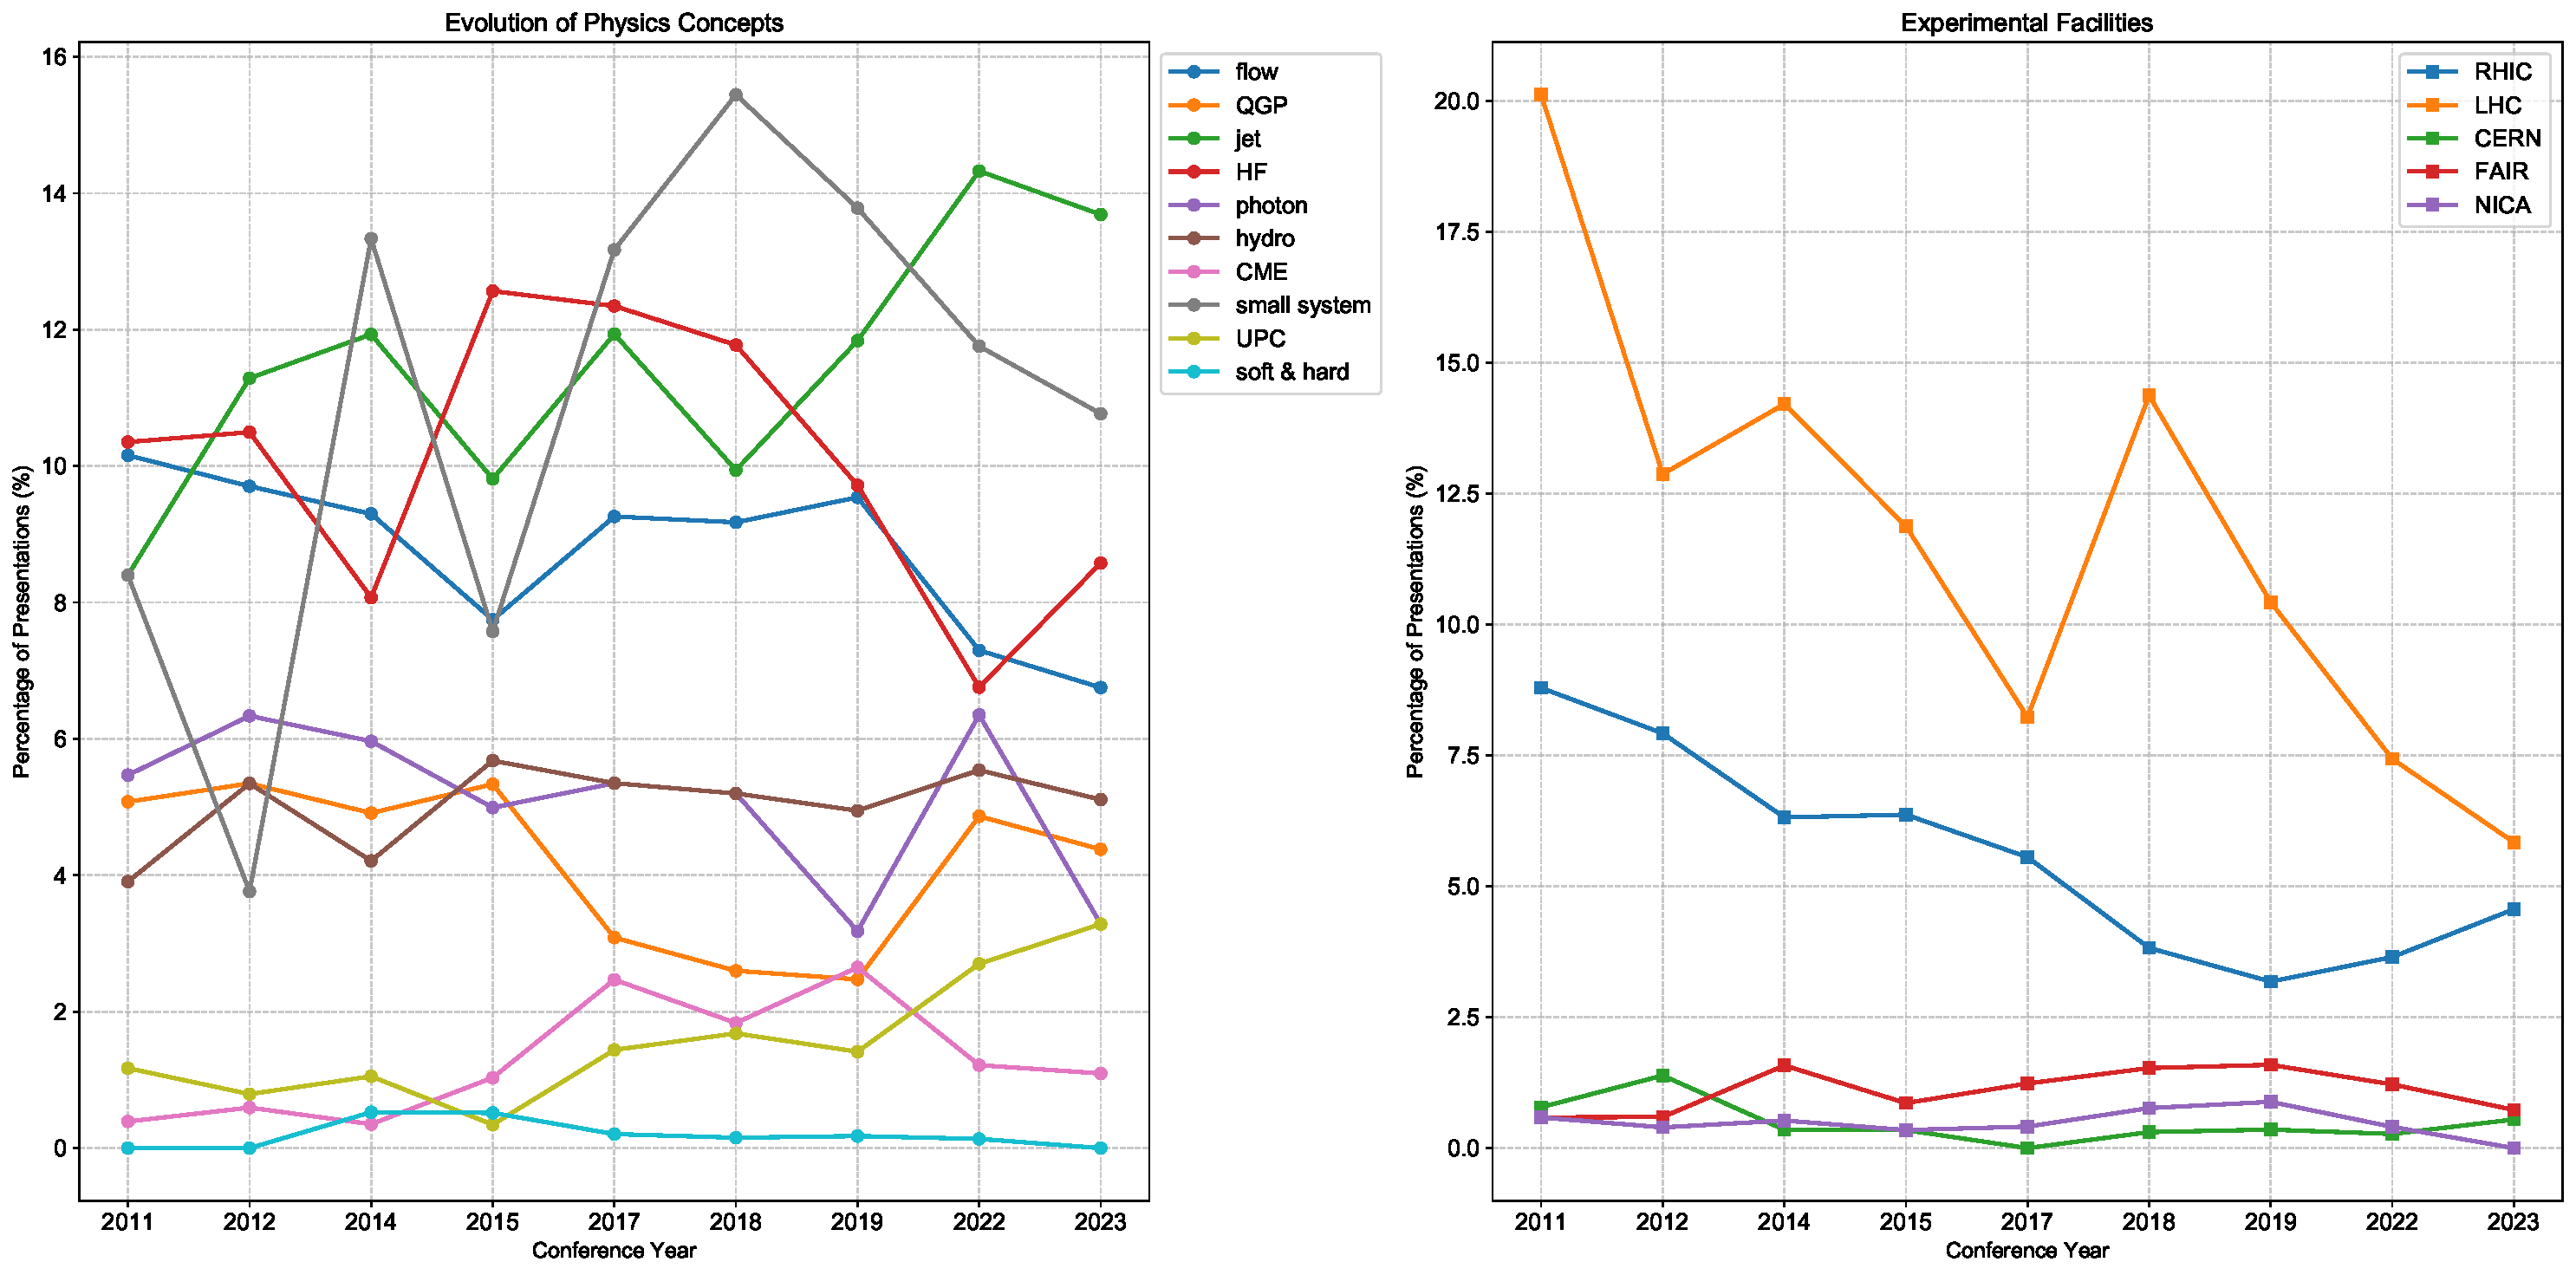
\includegraphics[width=\textwidth]{figures/QM_keyword_analysis.pdf}
\caption{Comprehensive analysis of research topics in Quark Matter conferences from 2011 to 2023. The top panels show the evolution of key physics concepts (left) and experimental facilities (right) as percentages of total presentations. The bottom panels display word clouds for each conference year, highlighting the most prominent terms in presentation titles after removing common stopwords. This multi-faceted visualization reveals both quantitative trends and qualitative shifts in research focus over time.}
\label{fig:keywords}
\end{figure}

Figure~\ref{fig:keywords} presents a comprehensive analysis of research topics across Quark Matter conferences from 2011 to 2023. This enhanced visualization combines quantitative trend analysis with qualitative word clouds to provide deeper insights into the field's evolution:

The upper-left panel tracks specific physics concepts over time, revealing clear temporal patterns in research focus. "QGP \& Plasma" terms maintain a consistent presence throughout the period, confirming the central role of quark-gluon plasma studies in the field. However, we observe distinct phases in other research areas: "Flow \& Collectivity" shows peak interest in the middle years (2014-2018), while "Small Systems" and "Fluctuations" gain prominence in later conferences, reflecting the community's expanding research horizons.

The upper-right panel monitors mentions of experimental facilities, documenting the field's transition from facility-focused to phenomenon-focused research. Early conferences show strong emphasis on LHC and RHIC facilities, with a gradual decline in facility mentions as the research community moved toward more specific physical phenomena and measurements. The increasing mentions of future facilities in recent years (EIC, FAIR, NICA) signals the field's forward-looking perspective and preparation for next-generation experiments.

The word clouds for individual conference years provide qualitative context for these trends, highlighting the most distinctive terms after removing common stopwords. In our analysis, we deliberately filtered out trivial keywords that appear frequently but provide little insight into research trends. Terms such as "quark," "matter," "collision," "heavy-ion," "measurement," "study," and "analysis" were removed despite their high frequency, as they represent generic terminology common to all presentations rather than indicators of specific research directions. This filtering process allows the visualization to highlight meaningful physics concepts and emerging research areas that would otherwise be obscured by these ubiquitous terms.

These visualizations reveal subtle shifts in terminology and emphasis that complement the quantitative analysis. For instance, we can observe the emergence of terms related to machine learning and computational approaches in more recent conferences, reflecting the field's adoption of new analytical techniques.

Theoretical evolution is also evident in the changing prominence of terms across years. Early conferences feature more general theoretical frameworks, while later years show increasing specificity in theoretical approaches, suggesting growing theoretical sophistication and specialization as the field matures.

This multi-faceted keyword analysis provides a data-driven view of how research priorities in the heavy-ion physics community have evolved over the past decade and points to potential future directions as indicated by emerging keywords in recent conferences.

\subsection{Geographical Distribution of Contributions}

\begin{figure}[H]
\centering
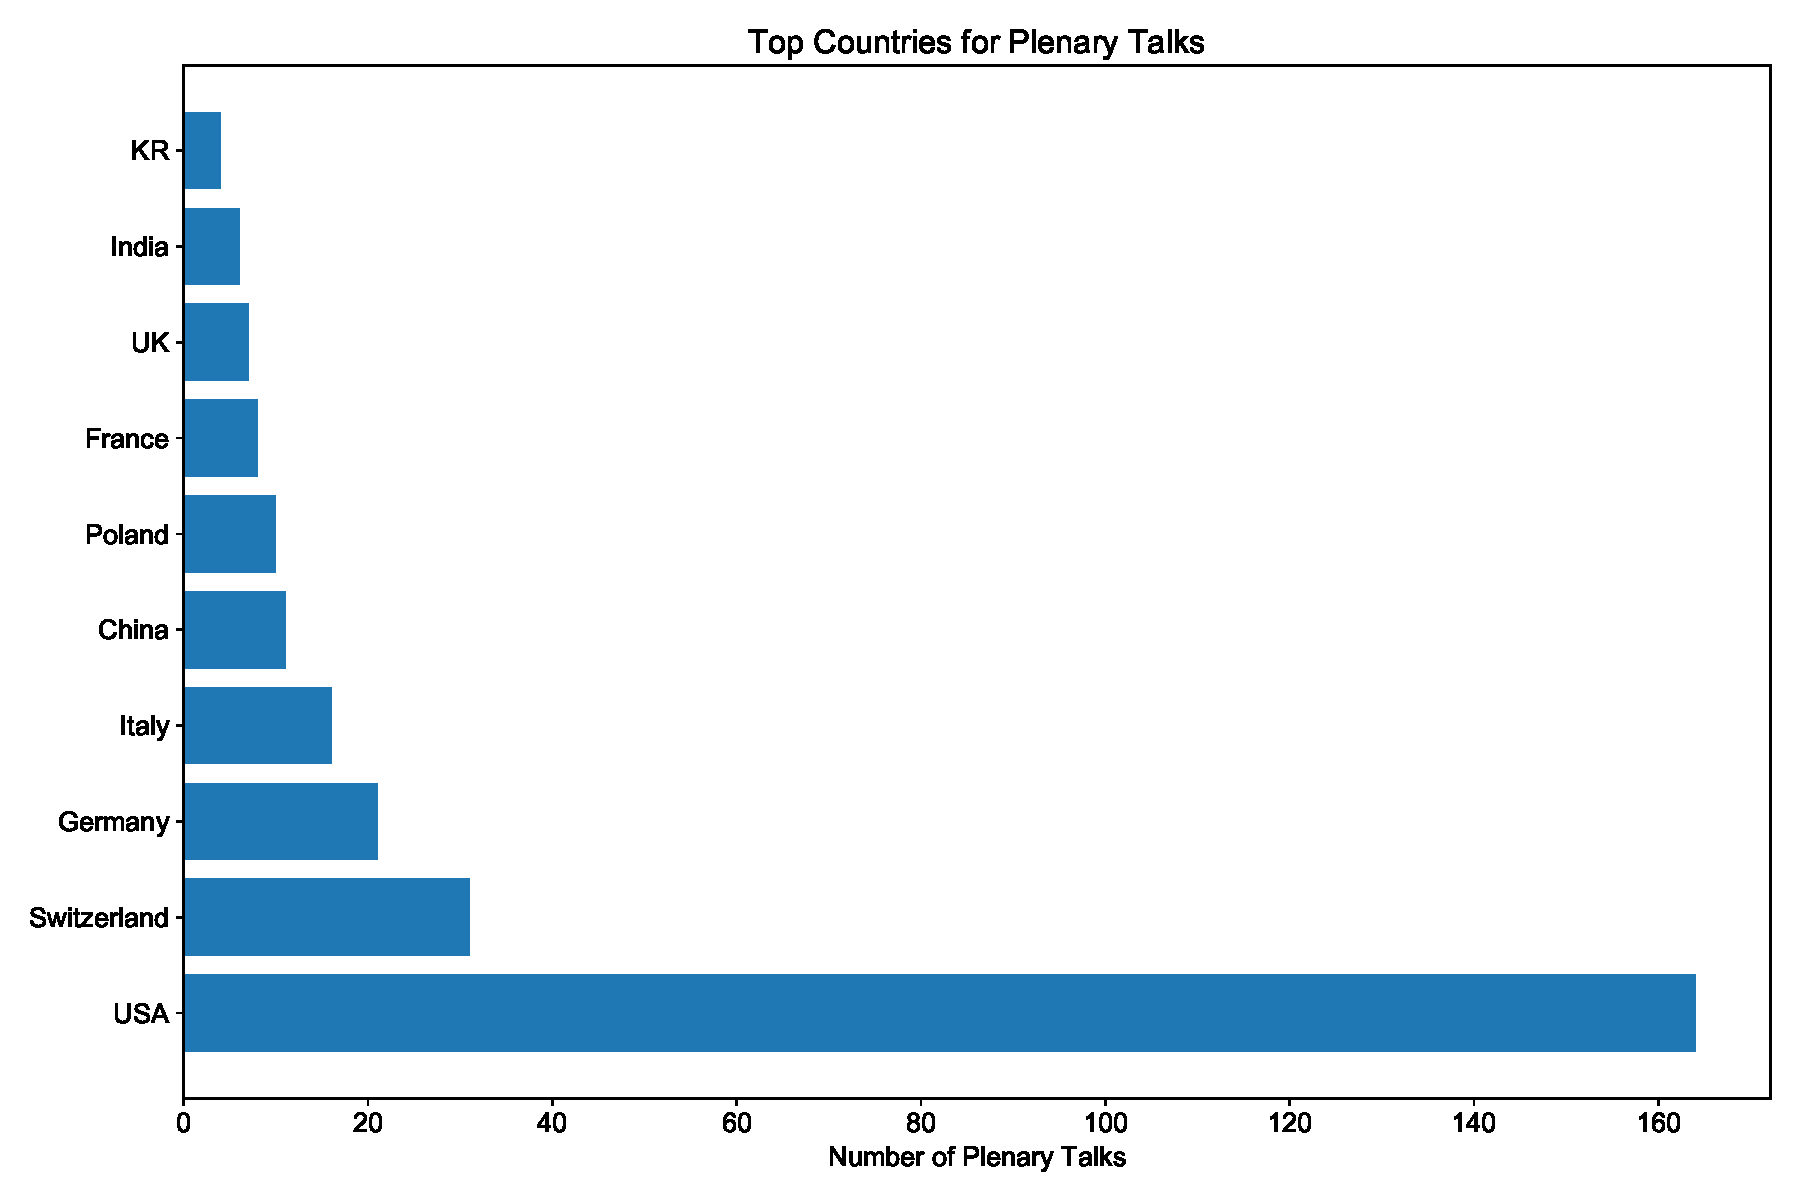
\includegraphics[width=\textwidth]{figures/plenary_talks_by_country.pdf}
\caption{Distribution of plenary talks by country across Quark Matter conferences from 2011 to 2025. The horizontal bars show the number of plenary presentations given by speakers from each of the top 15 countries, with percentage labels indicating relative contribution. Countries are color-coded by region for better geographical context. This enhanced visualization reveals both dominant contributors and emerging participants in high-visibility presentations. The data quality has been significantly improved through our comprehensive affiliation resolution system, which resolved missing country information for nearly 97\% of all presentations.}
\label{fig:country_plenary}
\end{figure}

Figure~\ref{fig:country_plenary} displays the distribution of plenary talks by country across Quark Matter conferences. Plenary talks represent the highest visibility presentations at these conferences and are typically allocated to highlight significant advances in the field. Several important patterns are evident:

There is a consistent dominance by a small number of countries, particularly the United States, which maintains a substantial share of plenary talks across all conference years. This reflects the significant investment in heavy-ion research infrastructure and personnel in the US, home to the RHIC facility and major ALICE, CMS, and ATLAS heavy-ion programs.

European countries collectively represent another major block, with Germany, France, and the UK consistently present. The distribution among European countries shows some variability between conferences, potentially reflecting both the location of the conference (European conferences tend to have more European speakers) and shifts in research output.

Asian representation, particularly from China, Japan, and India, shows interesting dynamics over time. We observe a general trend of increasing representation from these countries, especially in more recent conferences, reflecting growing investment in the field in these regions.

Emerging contributors such as Brazil, South Africa, and Poland are now visible in the expanded visualization, showing how the field is gradually becoming more internationally diverse even as traditional centers maintain their prominent positions.

The data reveals potential geographical imbalances in high-visibility speaking opportunities. While some variation is expected due to differences in community size and research output, the persistence of these patterns may warrant attention from conference organizers interested in ensuring equitable international representation.

\begin{figure}[H]
\centering
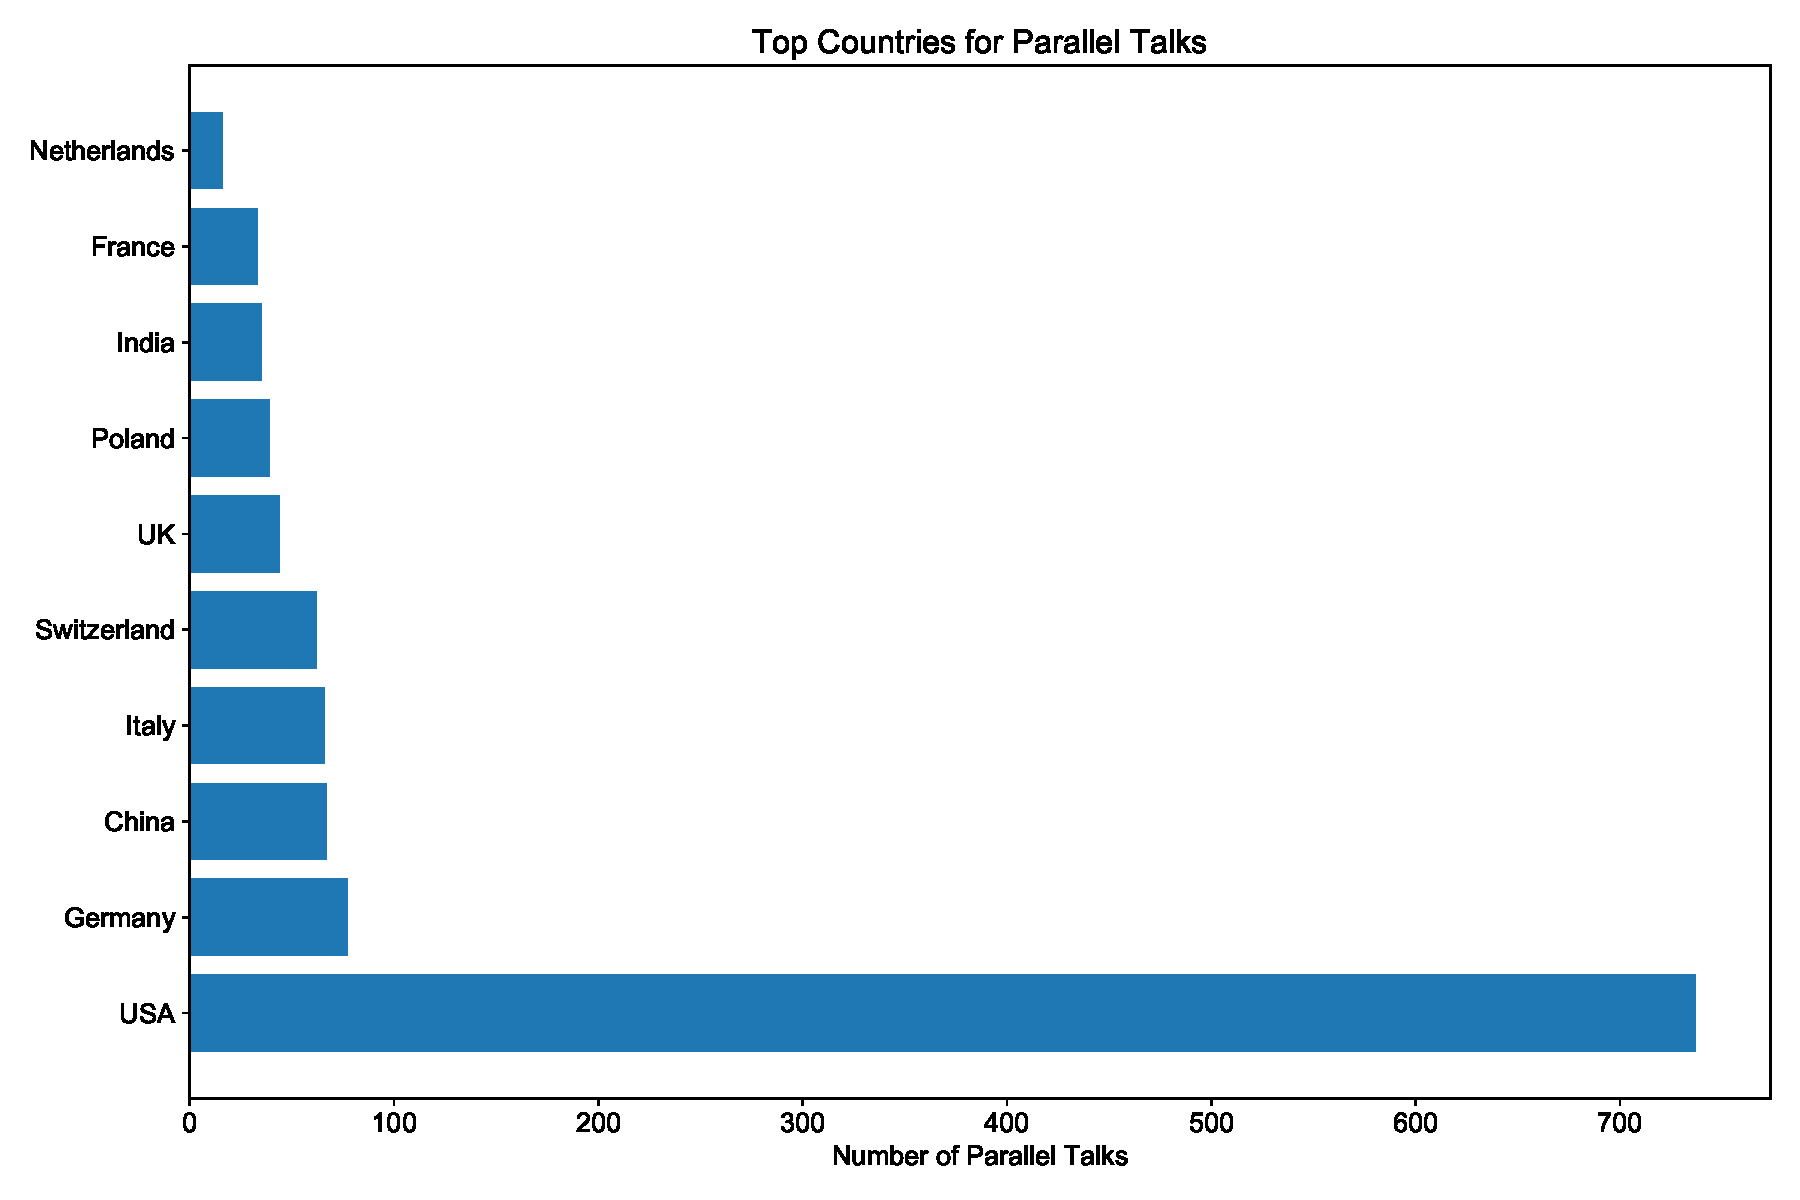
\includegraphics[width=\textwidth]{figures/parallel_talks_by_country.pdf}
\caption{Distribution of parallel talks by country across Quark Matter conferences from 2011 to 2025. The horizontal bars show the number of parallel session presentations given by speakers from each of the top 15 countries, with percentage labels indicating their share of the total presentations. This expanded visualization reveals broader participation patterns compared to plenary talks and illustrates how research contributions are distributed globally, including both established and emerging contributors.}
\label{fig:country_parallel}
\end{figure}

Figure~\ref{fig:country_parallel} shows the distribution of parallel talks by country, providing insight into the broader participation patterns beyond the highly selective plenary sessions. Parallel talks represent the majority of oral presentations at Quark Matter conferences and offer a more comprehensive view of active research in the field:

The country distribution for parallel talks shows greater diversity compared to plenary talks, with more countries represented and somewhat more balanced proportions. This suggests that while plenary selections may favor established research groups from certain countries, the parallel sessions incorporate a wider geographical range of contributions.

We observe interesting temporal trends, with some countries showing increasing representation over time (e.g., China), while others maintain relatively stable participation. These trends likely reflect both changes in research output and evolving selection processes by conference organizers.

The correlation between conference location and country representation is somewhat visible in the parallel session data, with host countries typically showing increased representation in their conference years. This may reflect both practical considerations (travel funding) and deliberate efforts to showcase local research.

Despite the greater diversity, there remains a clear stratification, with a few countries consistently accounting for the majority of parallel talks. This pattern raises questions about structural factors affecting international participation, including funding disparities, language barriers, and access to research infrastructure.

\begin{figure}[H]
\centering
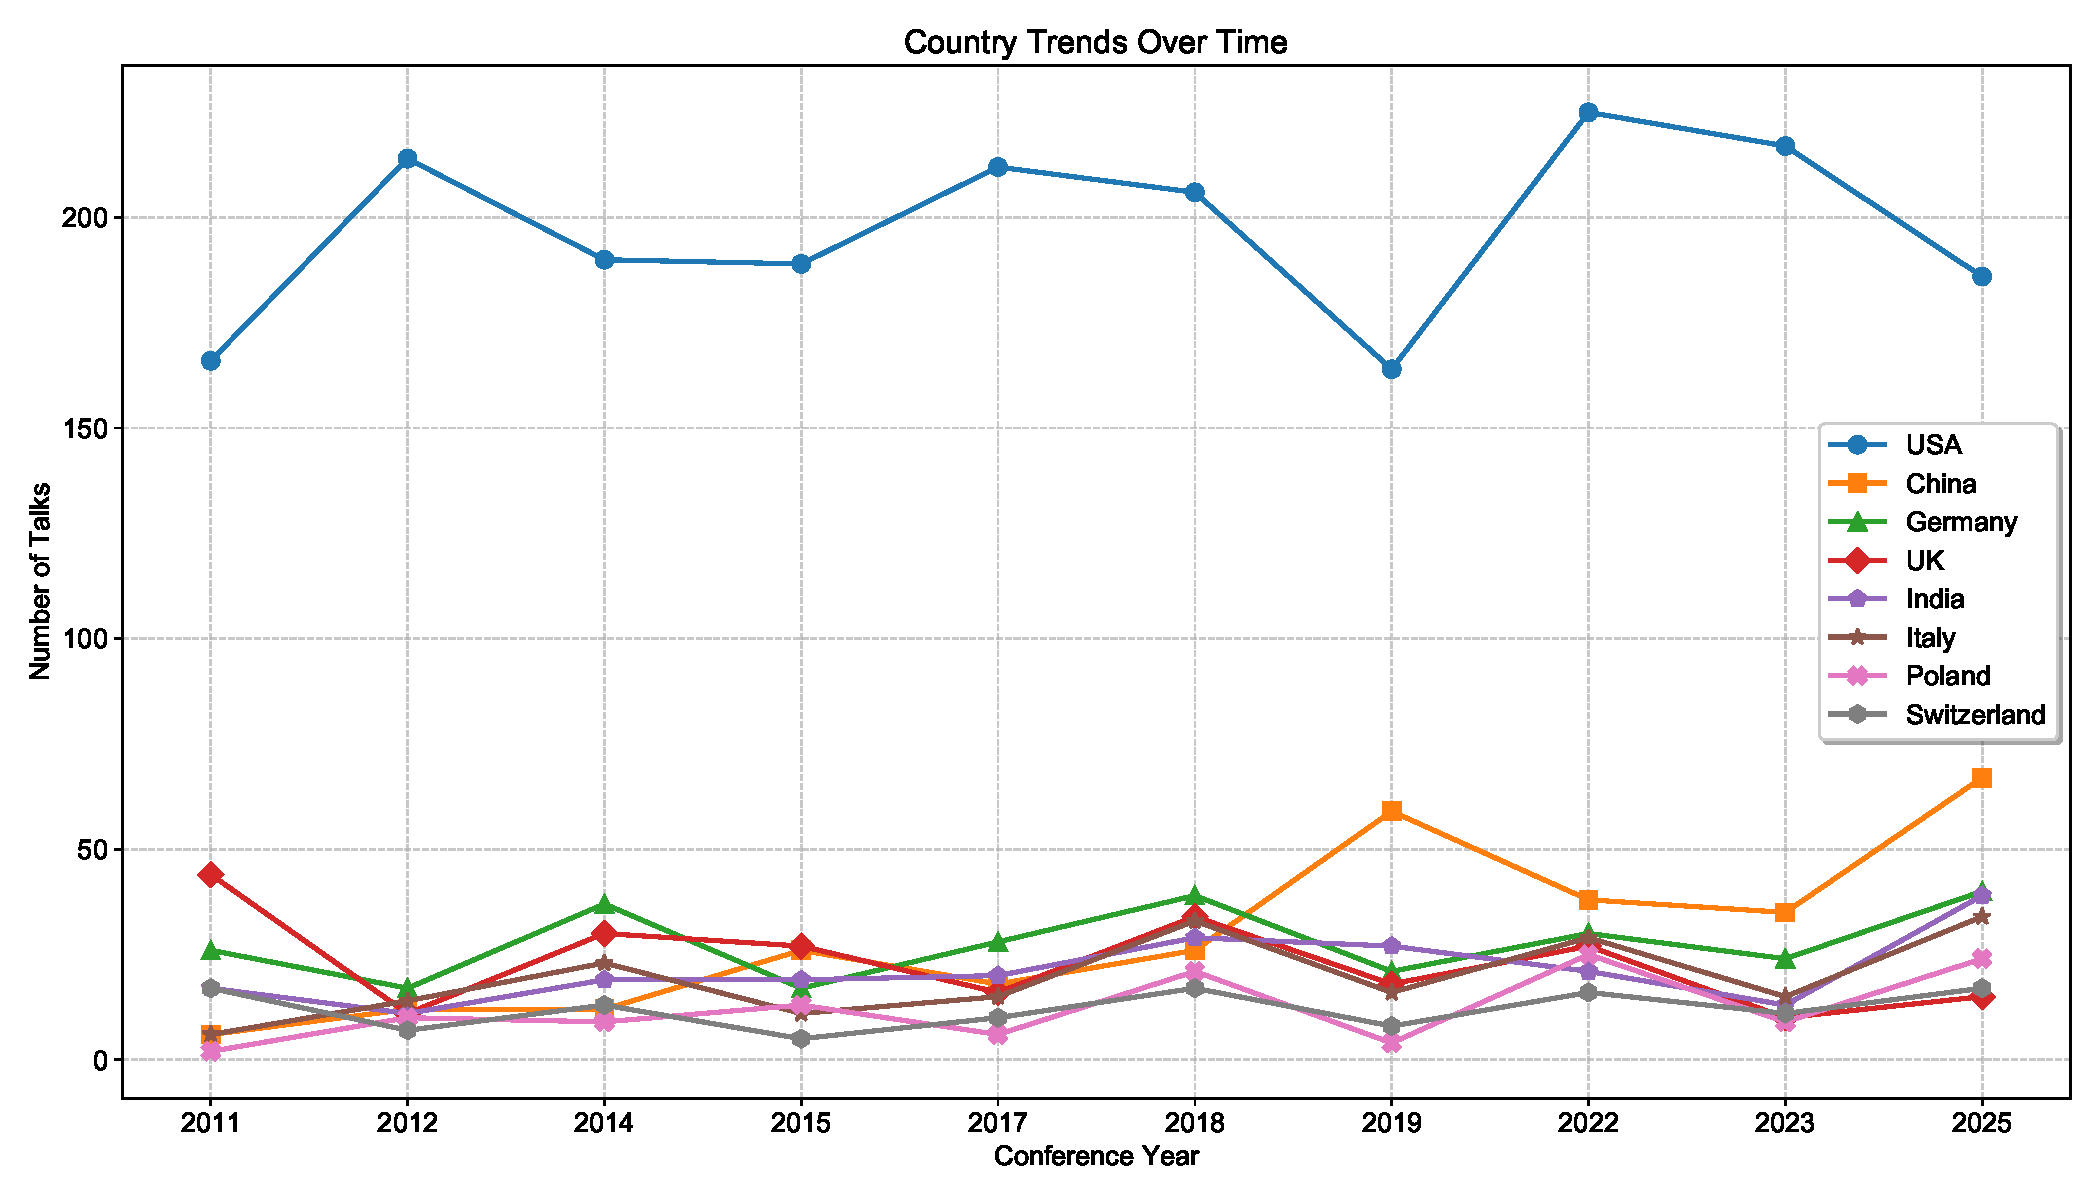
\includegraphics[width=\textwidth]{figures/country_trends_over_time.pdf}
\caption{Trends in country representation at Quark Matter conferences from 2011 to 2025. The line graph shows the percentage of total talks given by speakers from the top 8 countries (solid lines) and selected emerging countries (dashed lines) over time. This visualization reveals both persistent patterns of representation and changing dynamics as new countries increase their participation in the field.}
\label{fig:country_trends}
\end{figure}

Figure~\ref{fig:country_trends} provides a dynamic view of how country representation has evolved over time. This visualization offers valuable insights into both established patterns and emerging trends:

The top countries show relatively stable patterns of representation, with some year-to-year fluctuations often correlated with conference location. The United States and Germany consistently maintain strong representation, reflecting their established infrastructures and research programs.

Several emerging countries show noticeable upward trends, including Brazil, Poland, and Czech Republic. These trends highlight the gradual broadening of the field's geographical base, as heavy-ion physics research expands beyond its traditional centers.

The visualization reveals interesting patterns around conference years held in particular regions, where local representation typically increases. However, these location effects appear temporary rather than leading to sustained increases in representation from host countries.

This longitudinal view complements the aggregate analyses by revealing dynamics that might be obscured in cumulative statistics. The persistent gaps between established and emerging countries suggest that while progress is being made toward greater international diversity, significant disparities remain.

\subsection{Institutional Representation}

\begin{figure}[H]
\centering
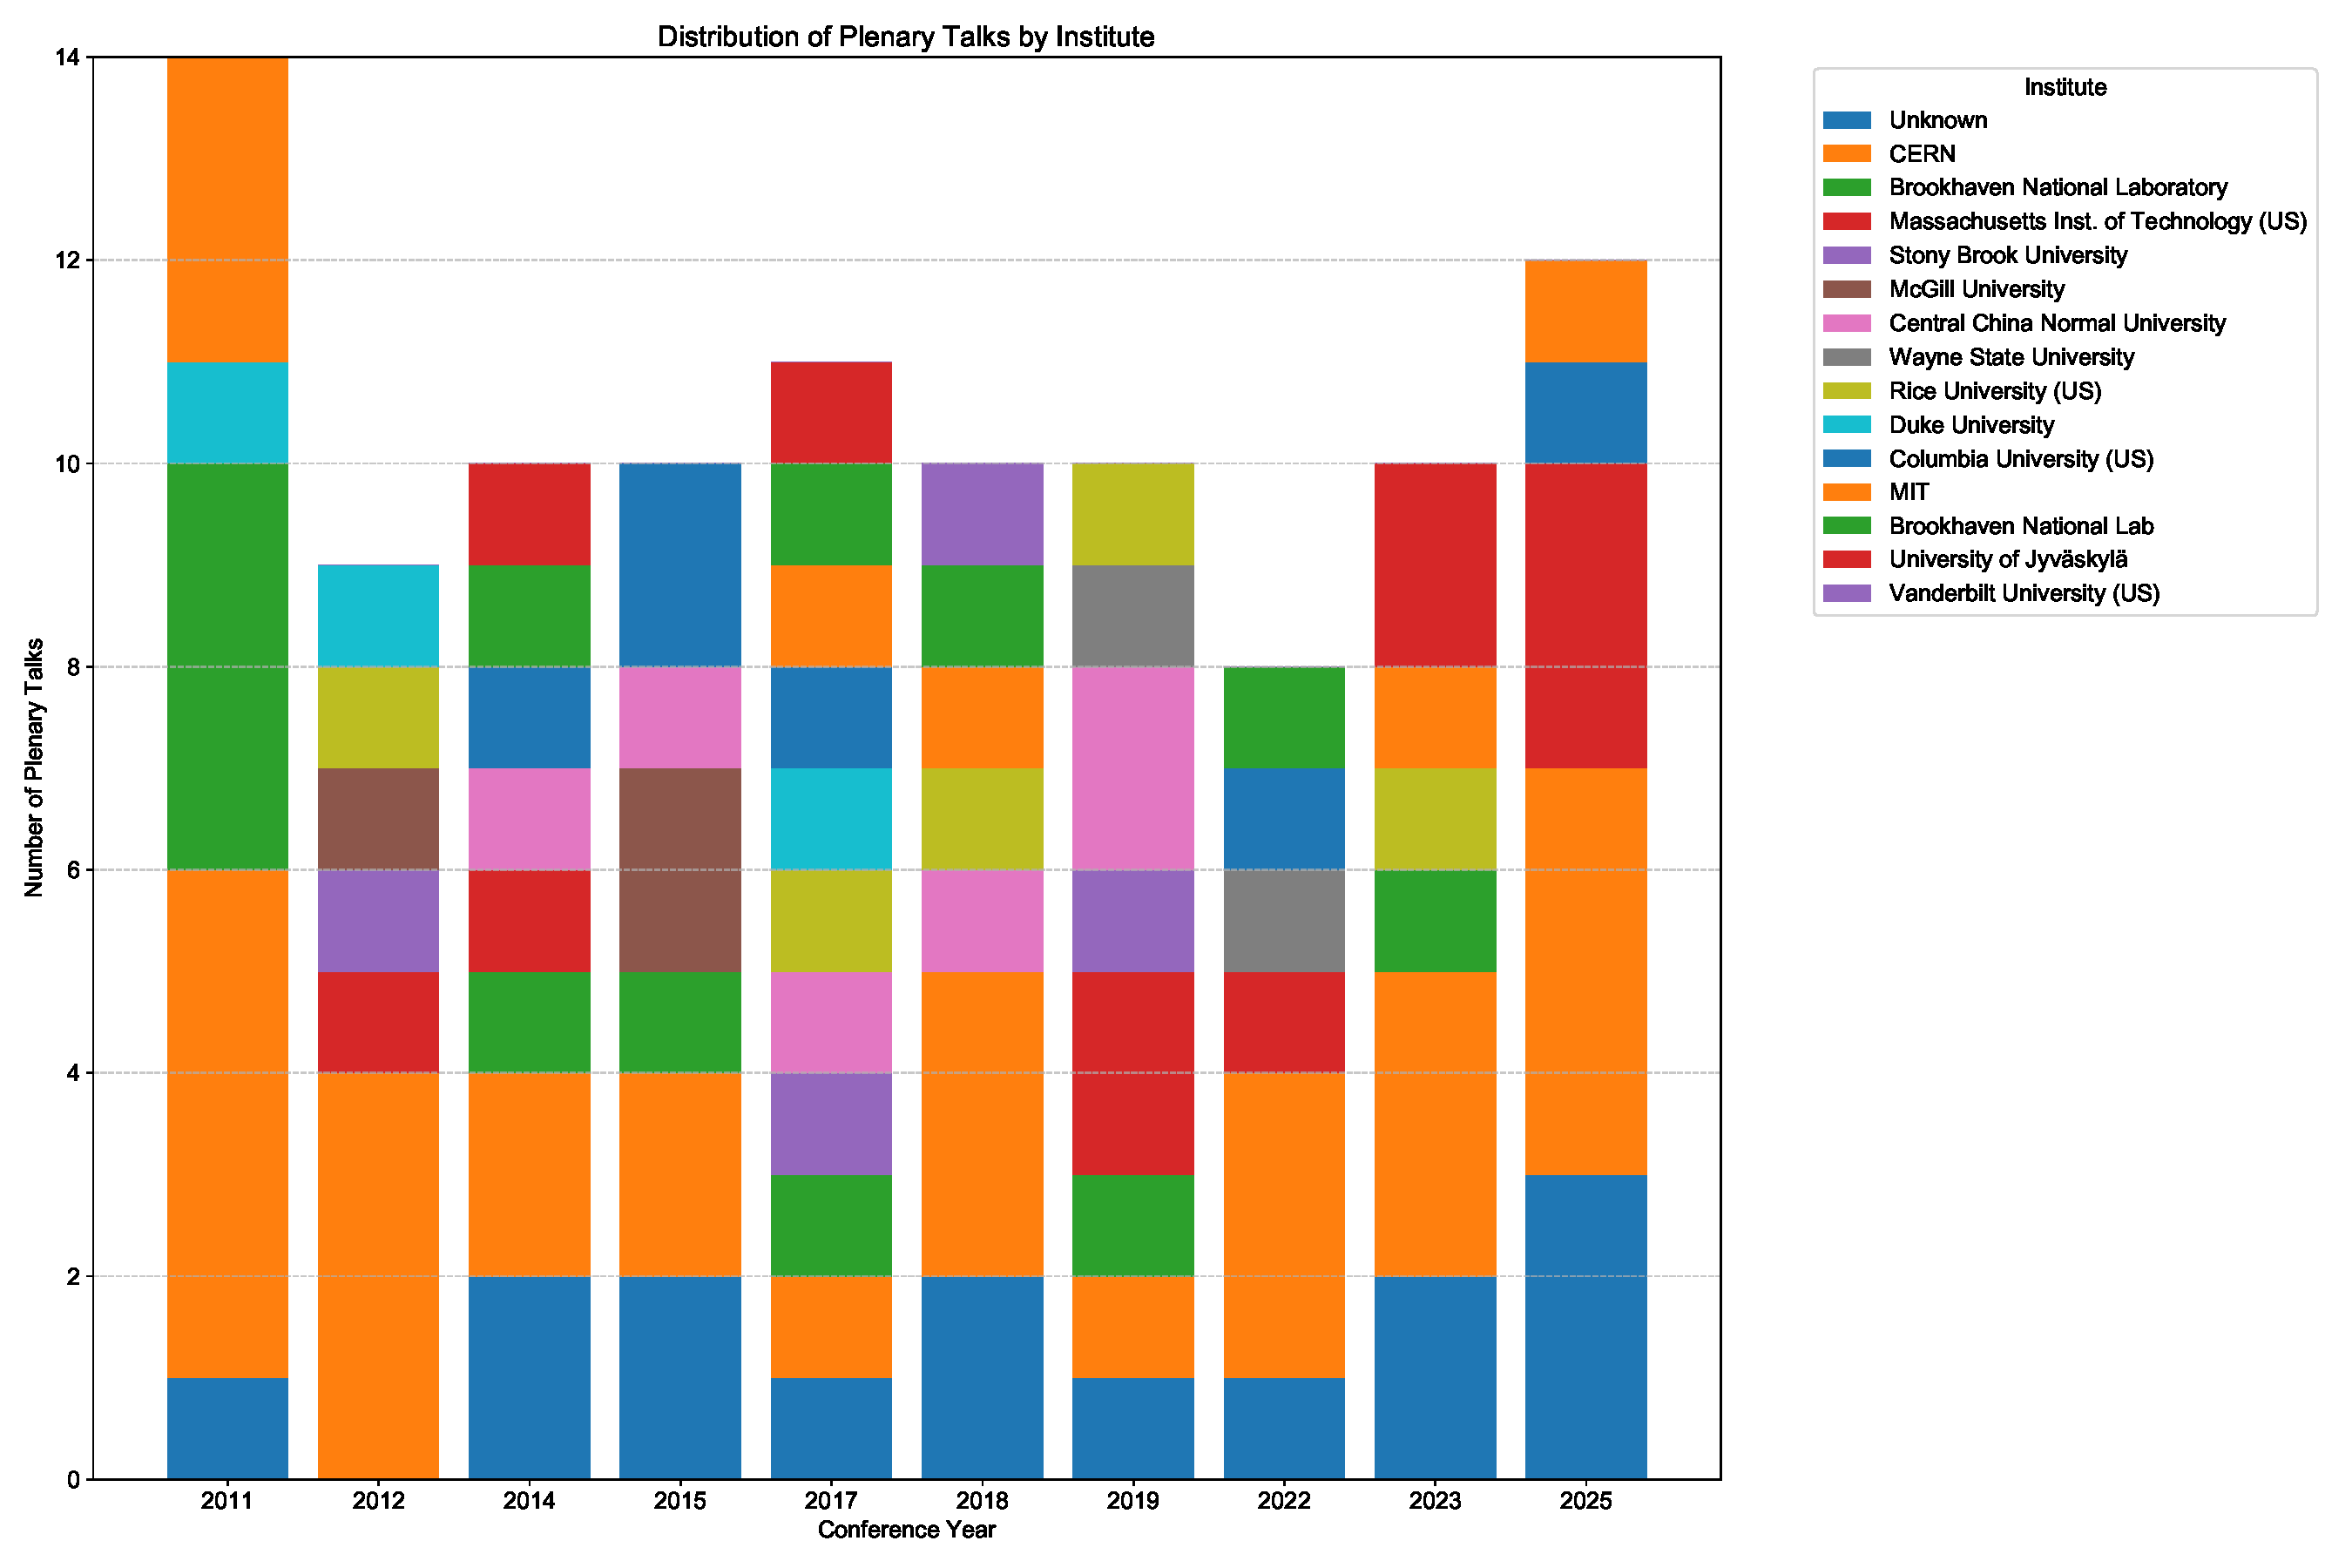
\includegraphics[width=\textwidth]{figures/plenary_talks_by_institute.pdf}
\caption{Distribution of plenary talks by institute across Quark Matter conferences from 2011 to 2025. The horizontal bars show the number of plenary presentations given by speakers from each of the top 20 institutes, with percentage labels indicating their relative contribution. Institutes are categorized by type (National Laboratory, University, Research Center) and sorted by total contribution. This expanded visualization reveals which research institutions have the most prominent representation in high-visibility speaking slots, highlighting potential concentration of influence in the field.}
\label{fig:institute_plenary}
\end{figure}

Figure~\ref{fig:institute_plenary} presents the distribution of plenary talks by research institute across Quark Matter conferences, offering insight into which institutions have the most significant presence in these high-visibility presentations:

The data reveals a strong concentration of plenary talks among a small group of elite research institutions, primarily major national laboratories and top-tier universities with strong nuclear physics programs. This concentration is even more pronounced than the country-level analysis, suggesting that institutional affiliation may be a more significant factor than nationality in plenary speaker selection.

Major experimental facilities hosts, such as Brookhaven National Laboratory (RHIC), CERN (LHC), and GSI (FAIR), are consistently well-represented, reflecting their central role in generating the data that drives the field forward. University representation is dominated by institutions with strong theoretical groups or significant roles in detector development and data analysis.

The temporal trends show some evolution in institutional representation, but the changes are relatively modest compared to the persistent dominance of established centers. New entrants to the "top institutes" list are rare across the conference series, suggesting limited mobility in the institutional hierarchy.

Mid-tier institutes now visible in our expanded visualization show interesting patterns of occasional representation, often correlating with specific breakthroughs or leadership in emerging research areas. This provides context for understanding how institutes beyond the dominant few gain visibility in the field.

These patterns raise important questions about how speaking opportunities, particularly high-visibility plenary talks, are allocated within the field. While meritocratic considerations certainly play a role, the strong institutional concentration may create barriers for researchers from less prestigious institutions to gain recognition for their work.

\begin{figure}[H]
\centering
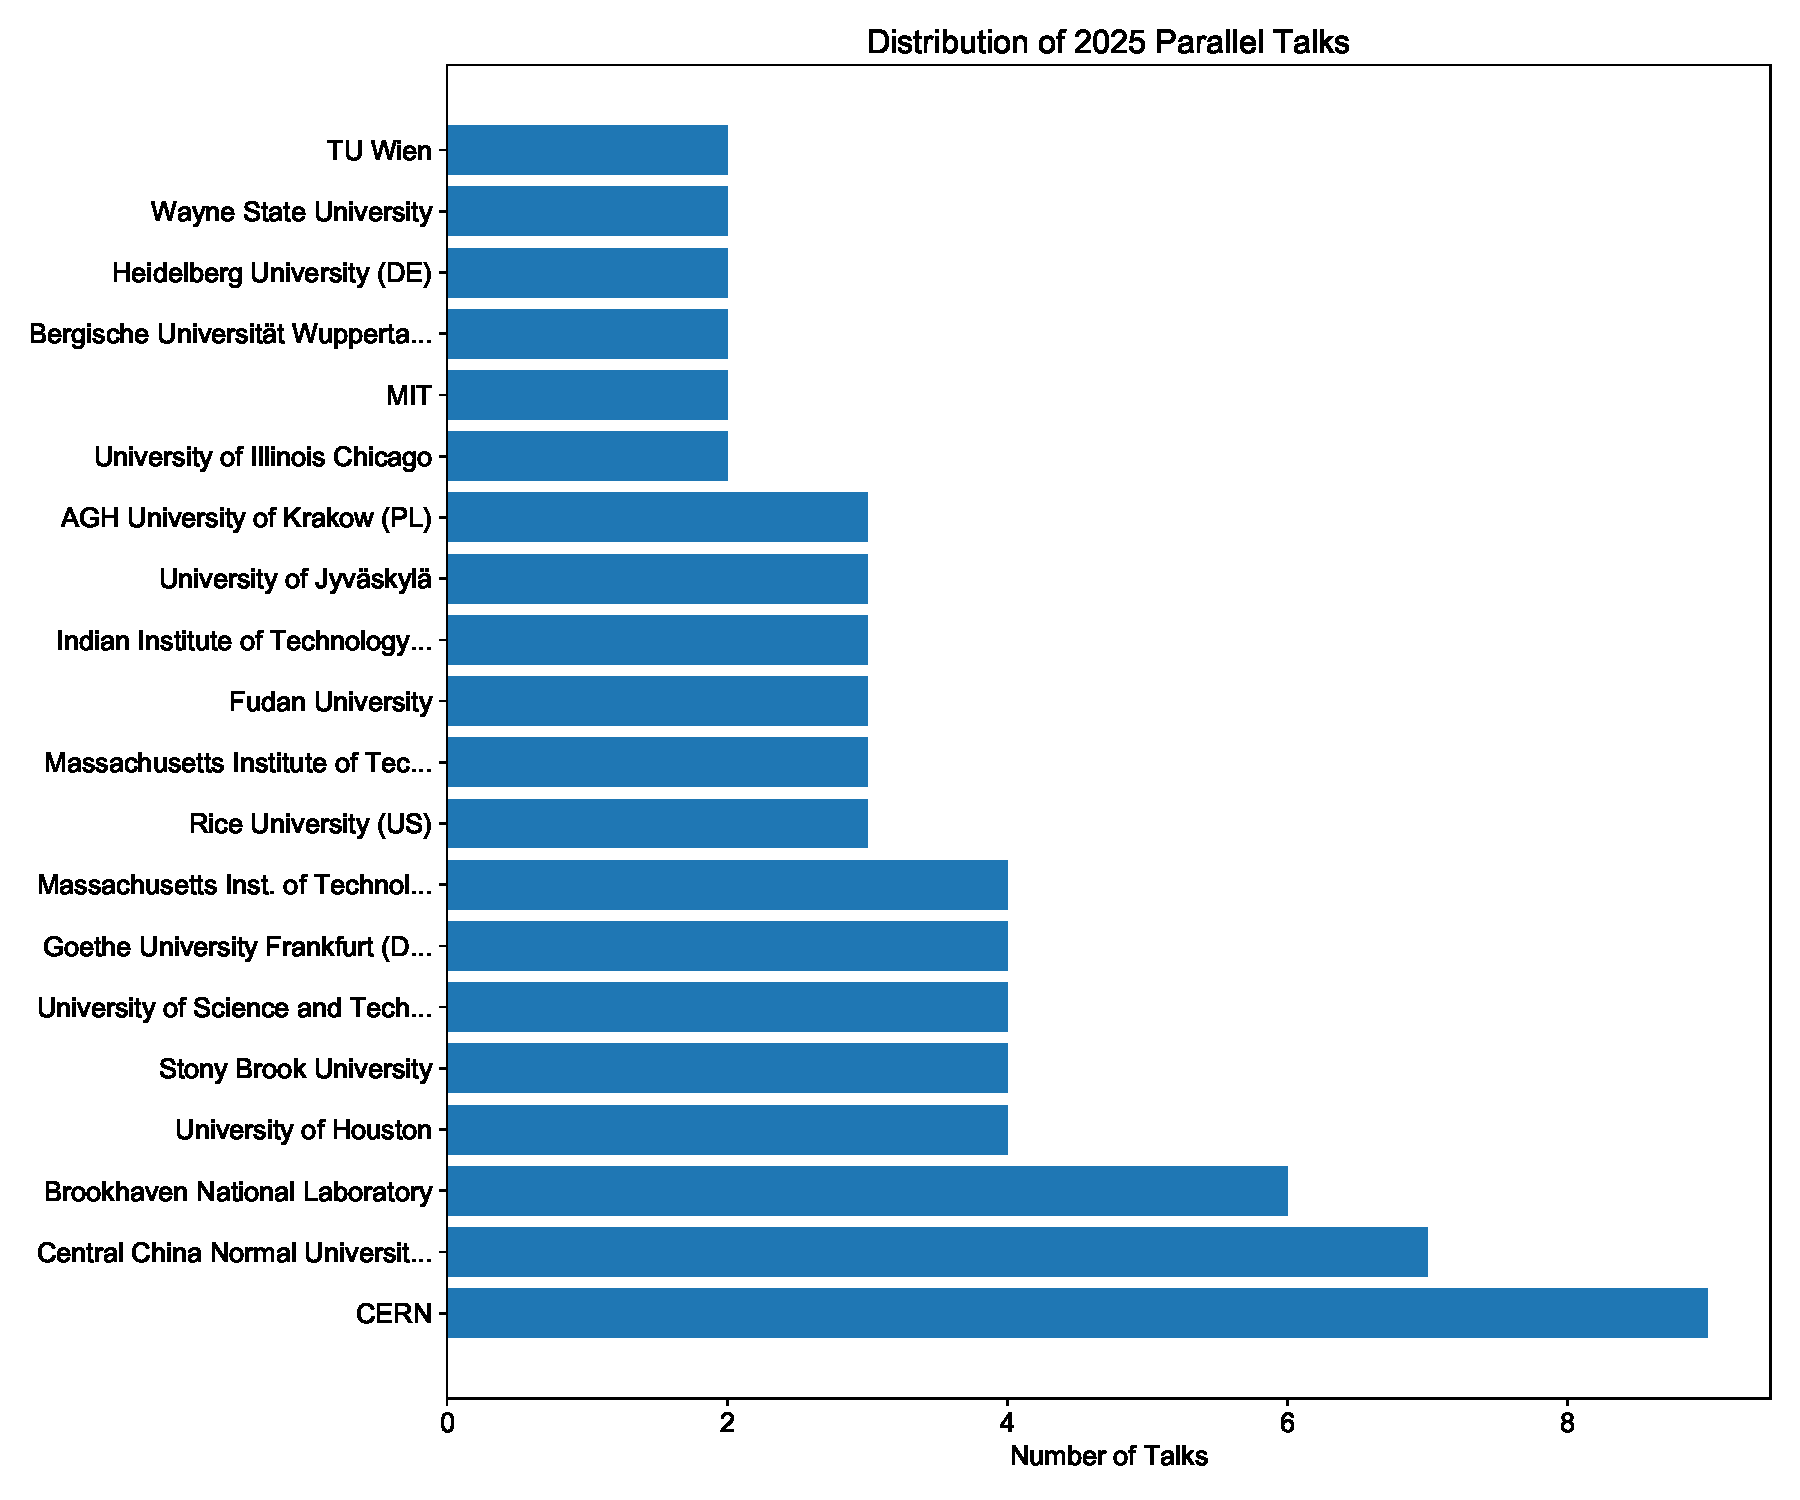
\includegraphics[width=\textwidth]{figures/parallel_talks_by_institute.pdf}
\caption{Distribution of parallel talks by institute across Quark Matter conferences from 2011 to 2025. The horizontal bars show the number of parallel session presentations given by speakers from each of the top 20 institutes, with percentage labels indicating their share of total presentations. Institutes are categorized by type and color-coded accordingly. This comprehensive visualization reveals broader institutional participation patterns compared to plenary talks and illustrates how research contributions are distributed across a wider range of research centers.}
\label{fig:institute_parallel}
\end{figure}

Figure~\ref{fig:institute_parallel} shows the distribution of parallel talks by institute, providing a broader view of institutional participation beyond the highly selective plenary sessions:

Similar to the country-level analysis, we observe greater institutional diversity in parallel sessions compared to plenary talks. While the leading institutions maintain strong representation, many more institutions participate at this level, creating a longer "tail" of participation that includes smaller universities and research groups.

The data shows some interesting dynamics in institutional participation over time. Some institutions show surges in certain years, often corresponding to significant experimental results or theoretical advances from those groups. Others maintain more consistent participation levels across the conference series.

Even in this broader participation category, there remains a clear stratification, with approximately 15-20 institutions accounting for a disproportionate share of all parallel talks. This concentration, while less extreme than for plenary talks, still suggests significant disparities in research visibility.

The institutional distribution also reflects the collaborative nature of the field, with participating institutions often clustered around major experimental collaborations (ALICE, STAR, PHENIX, etc.). Institutions with prominent roles in these collaborations typically secure more speaking slots, reflecting both their scientific contributions and their structural positions within the field.

\begin{figure}[H]
\centering
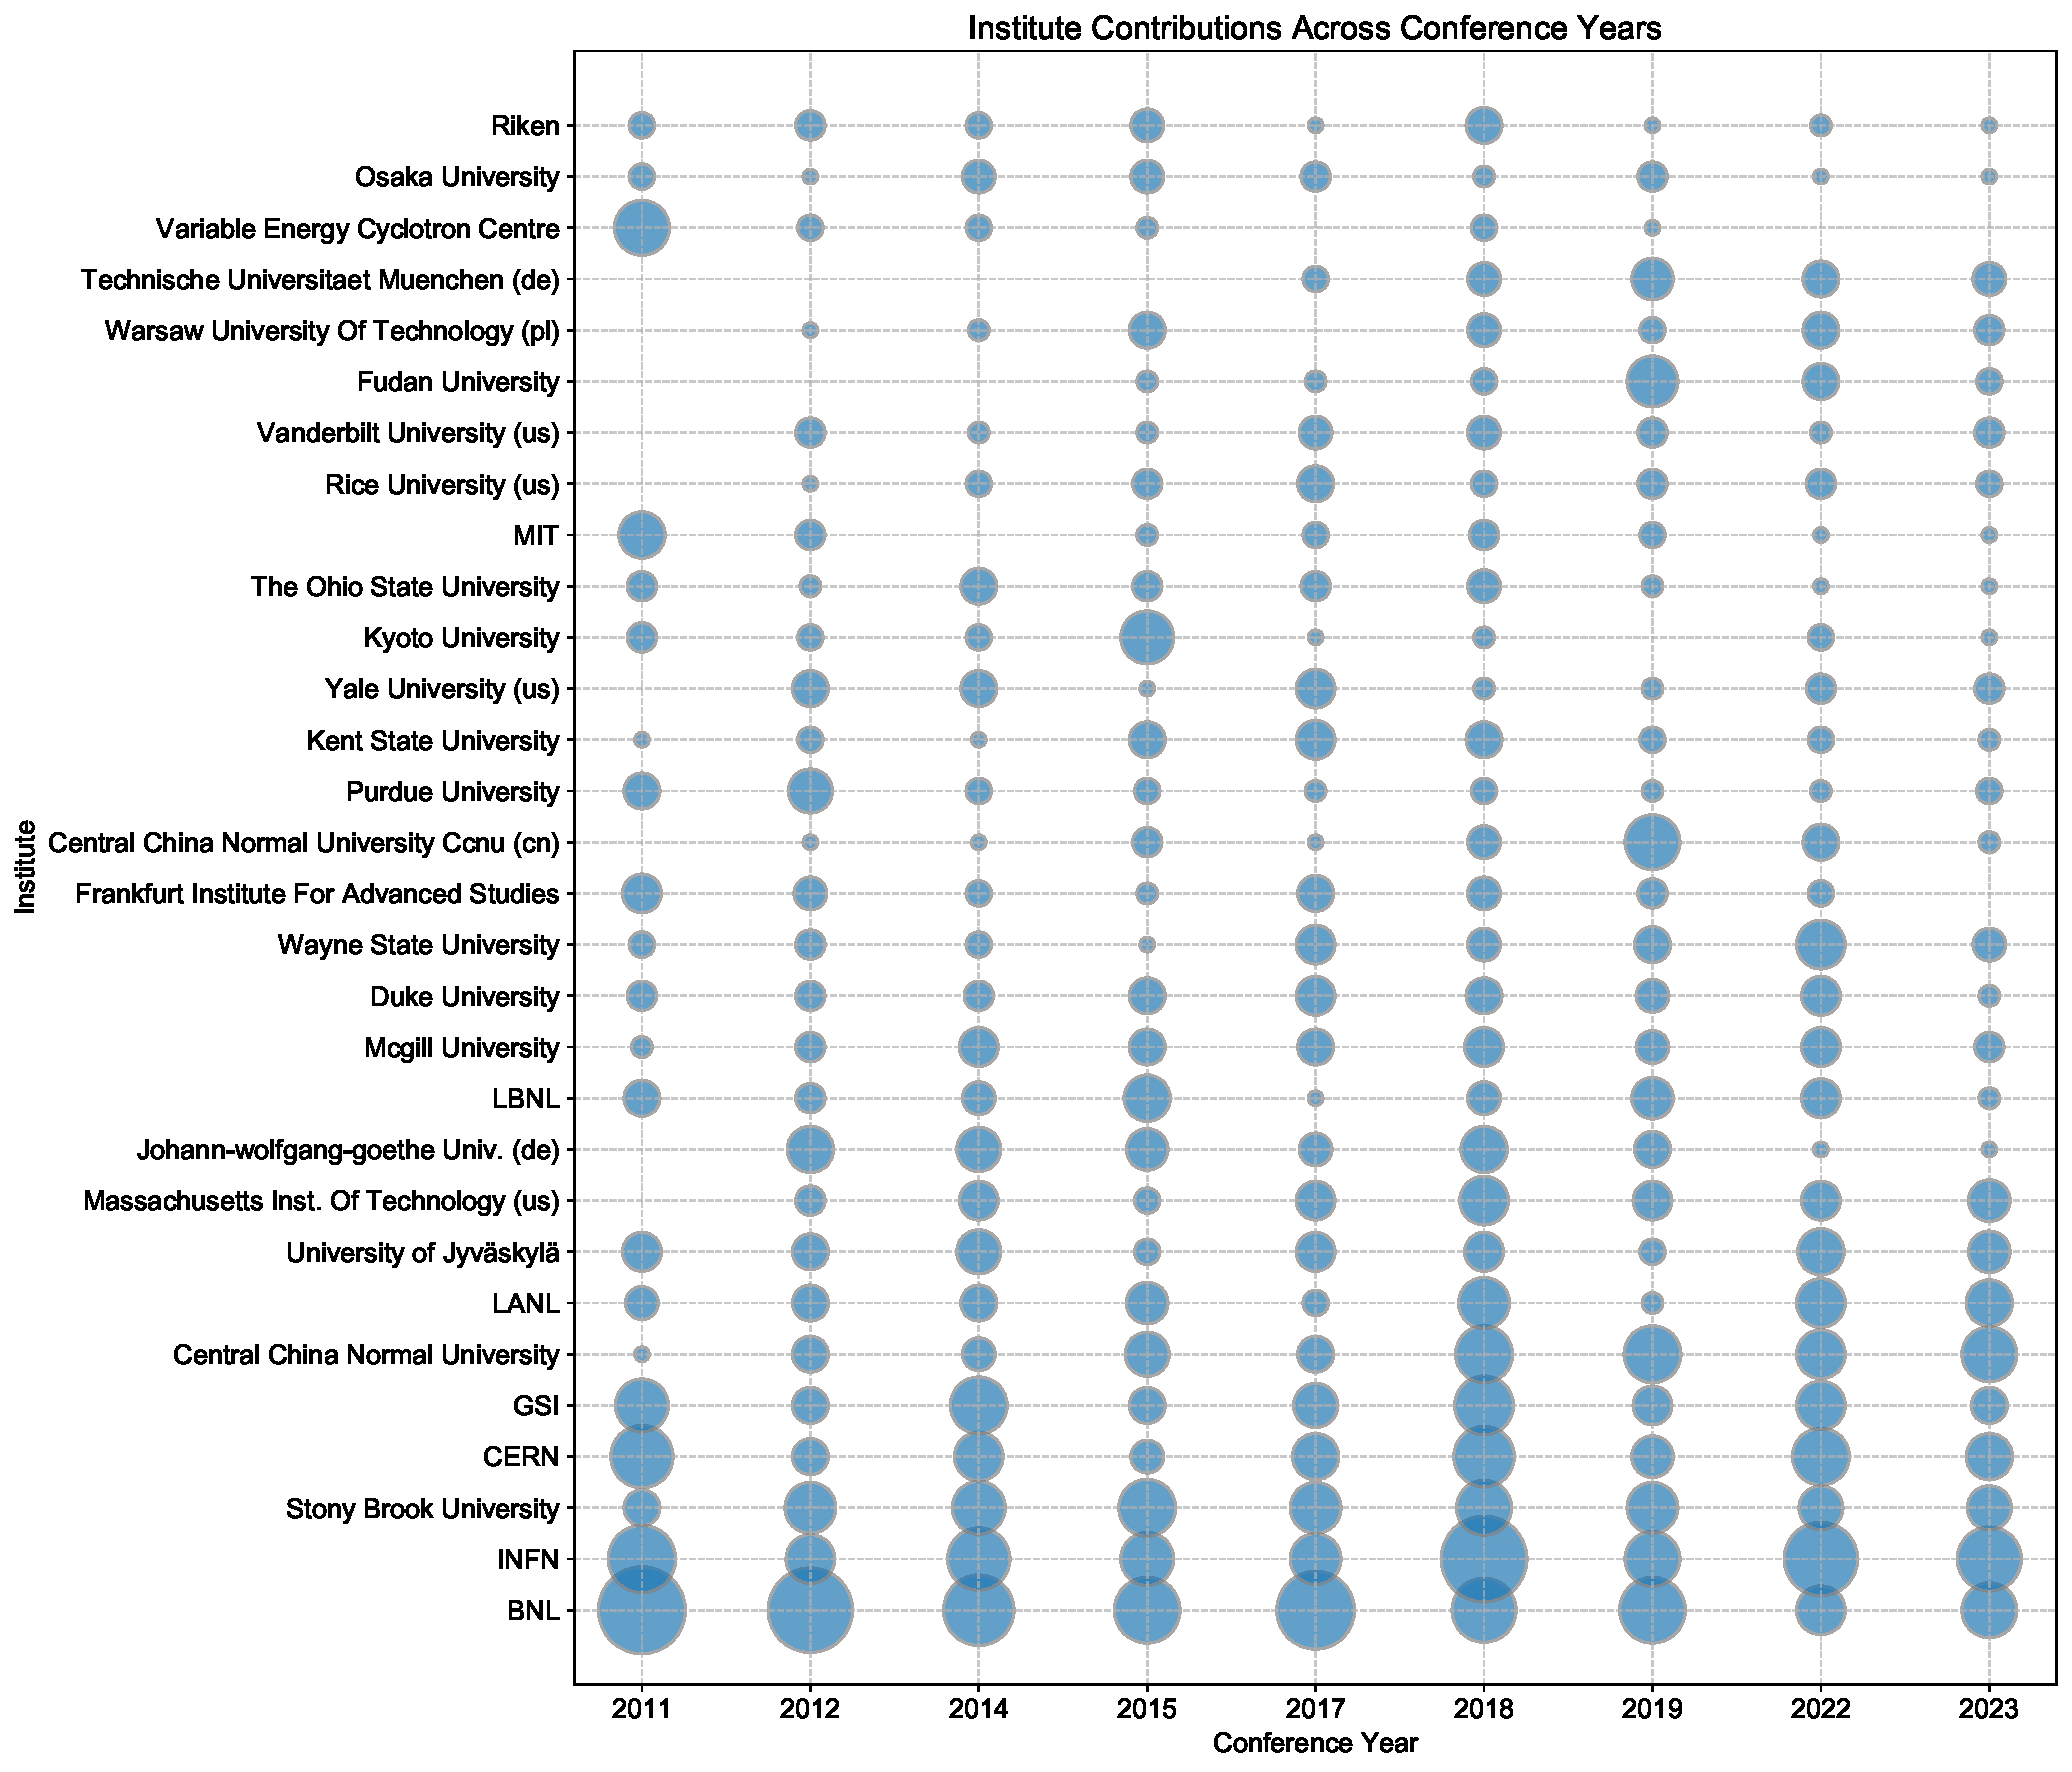
\includegraphics[width=\textwidth]{figures/institute_bubble_chart.pdf}
\caption{Institute contributions across Quark Matter conferences from 2011 to 2025. This bubble chart displays the presence and contribution volume of the top 30 institutes across conference years, with bubble size proportional to the number of presentations. This visualization reveals both consistently active institutions and those with intermittent but significant contributions, providing insight into how institutional participation patterns have evolved over time.}
\label{fig:institute_bubble}
\end{figure}

Figure~\ref{fig:institute_bubble} provides a novel perspective on institutional participation patterns through a time-series bubble chart. This visualization allows us to track the consistency and volume of contributions from the top 30 institutes across all conference years:

The chart reveals distinct participation patterns among institutes. Some maintain a consistent presence with relatively stable contribution volumes across all conferences, suggesting sustained research programs and established positions in the field. Others show more intermittent participation, with strong showings in specific years followed by reduced presence in others.

Major national laboratories (BNL, CERN) show some of the most consistent participation patterns, reflecting their central role in the experimental infrastructure that drives the field. University participation appears more variable, potentially reflecting shifting research priorities, funding cycles, or changes in research group composition.

Interestingly, some institutes show coordinated patterns, with increased participation in the same conference years. These correlations often align with major experimental runs or significant theoretical developments, highlighting how the field responds collectively to new opportunities and challenges.

The bubble chart also highlights emerging institutes that have increased their participation in more recent conferences, providing a window into the evolving institutional landscape of heavy-ion physics research. This longitudinal perspective complements the aggregate analyses by revealing dynamics that might be obscured in cumulative statistics.

\begin{figure}[H]
\centering
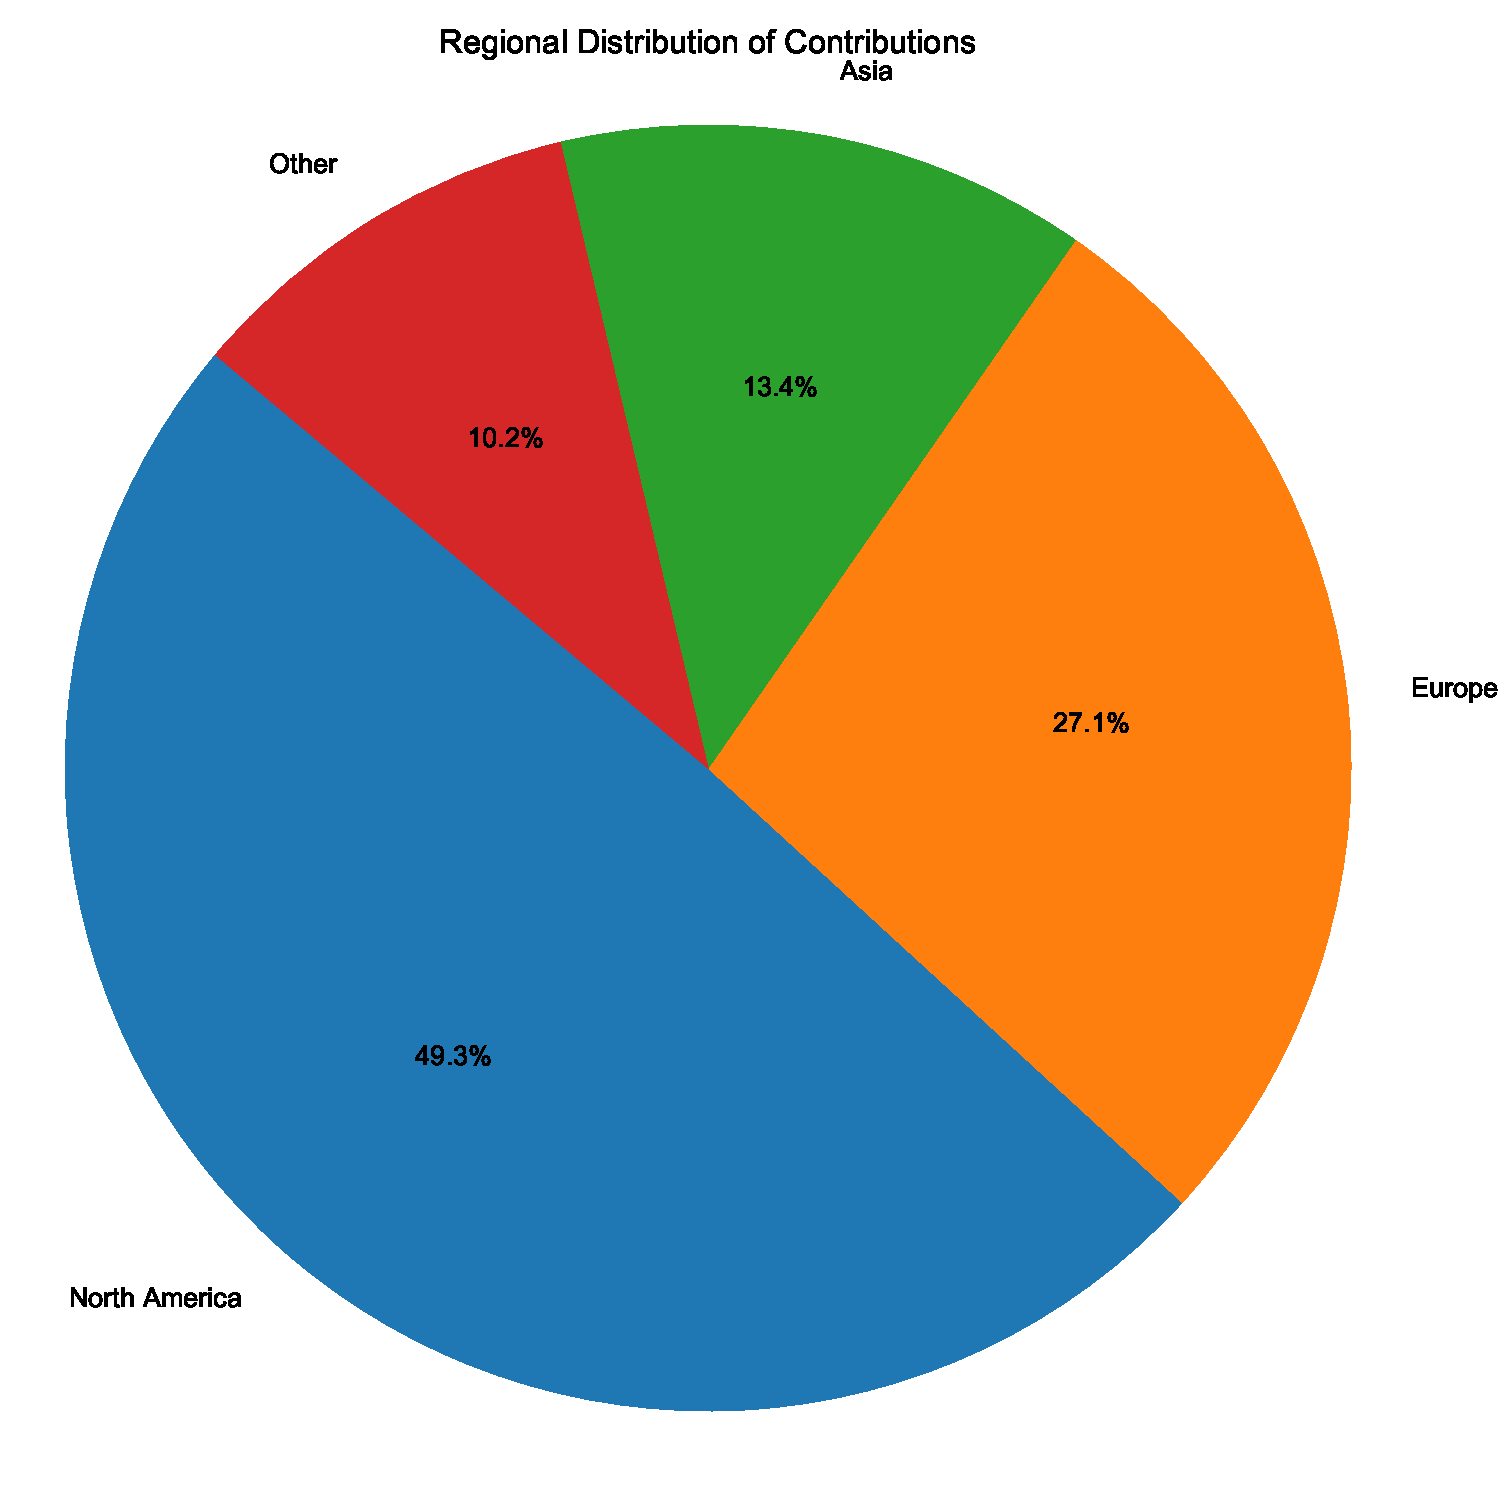
\includegraphics[width=\textwidth]{figures/regional_diversity.pdf}
\caption{Regional diversity of participation at Quark Matter conferences. The left panel shows the aggregate regional distribution of all contributions, while the right panel tracks how regional representation has evolved over time. Our improved affiliation matching methodology ensures that regional trends are based on more complete data, with less than 3\% of contributions having unknown origins. This visualization provides insight into the geographical spread of the heavy-ion physics community and highlights opportunities for increasing participation from underrepresented regions.}
\label{fig:regional_diversity}
\end{figure}

\begin{figure}[H]
\centering
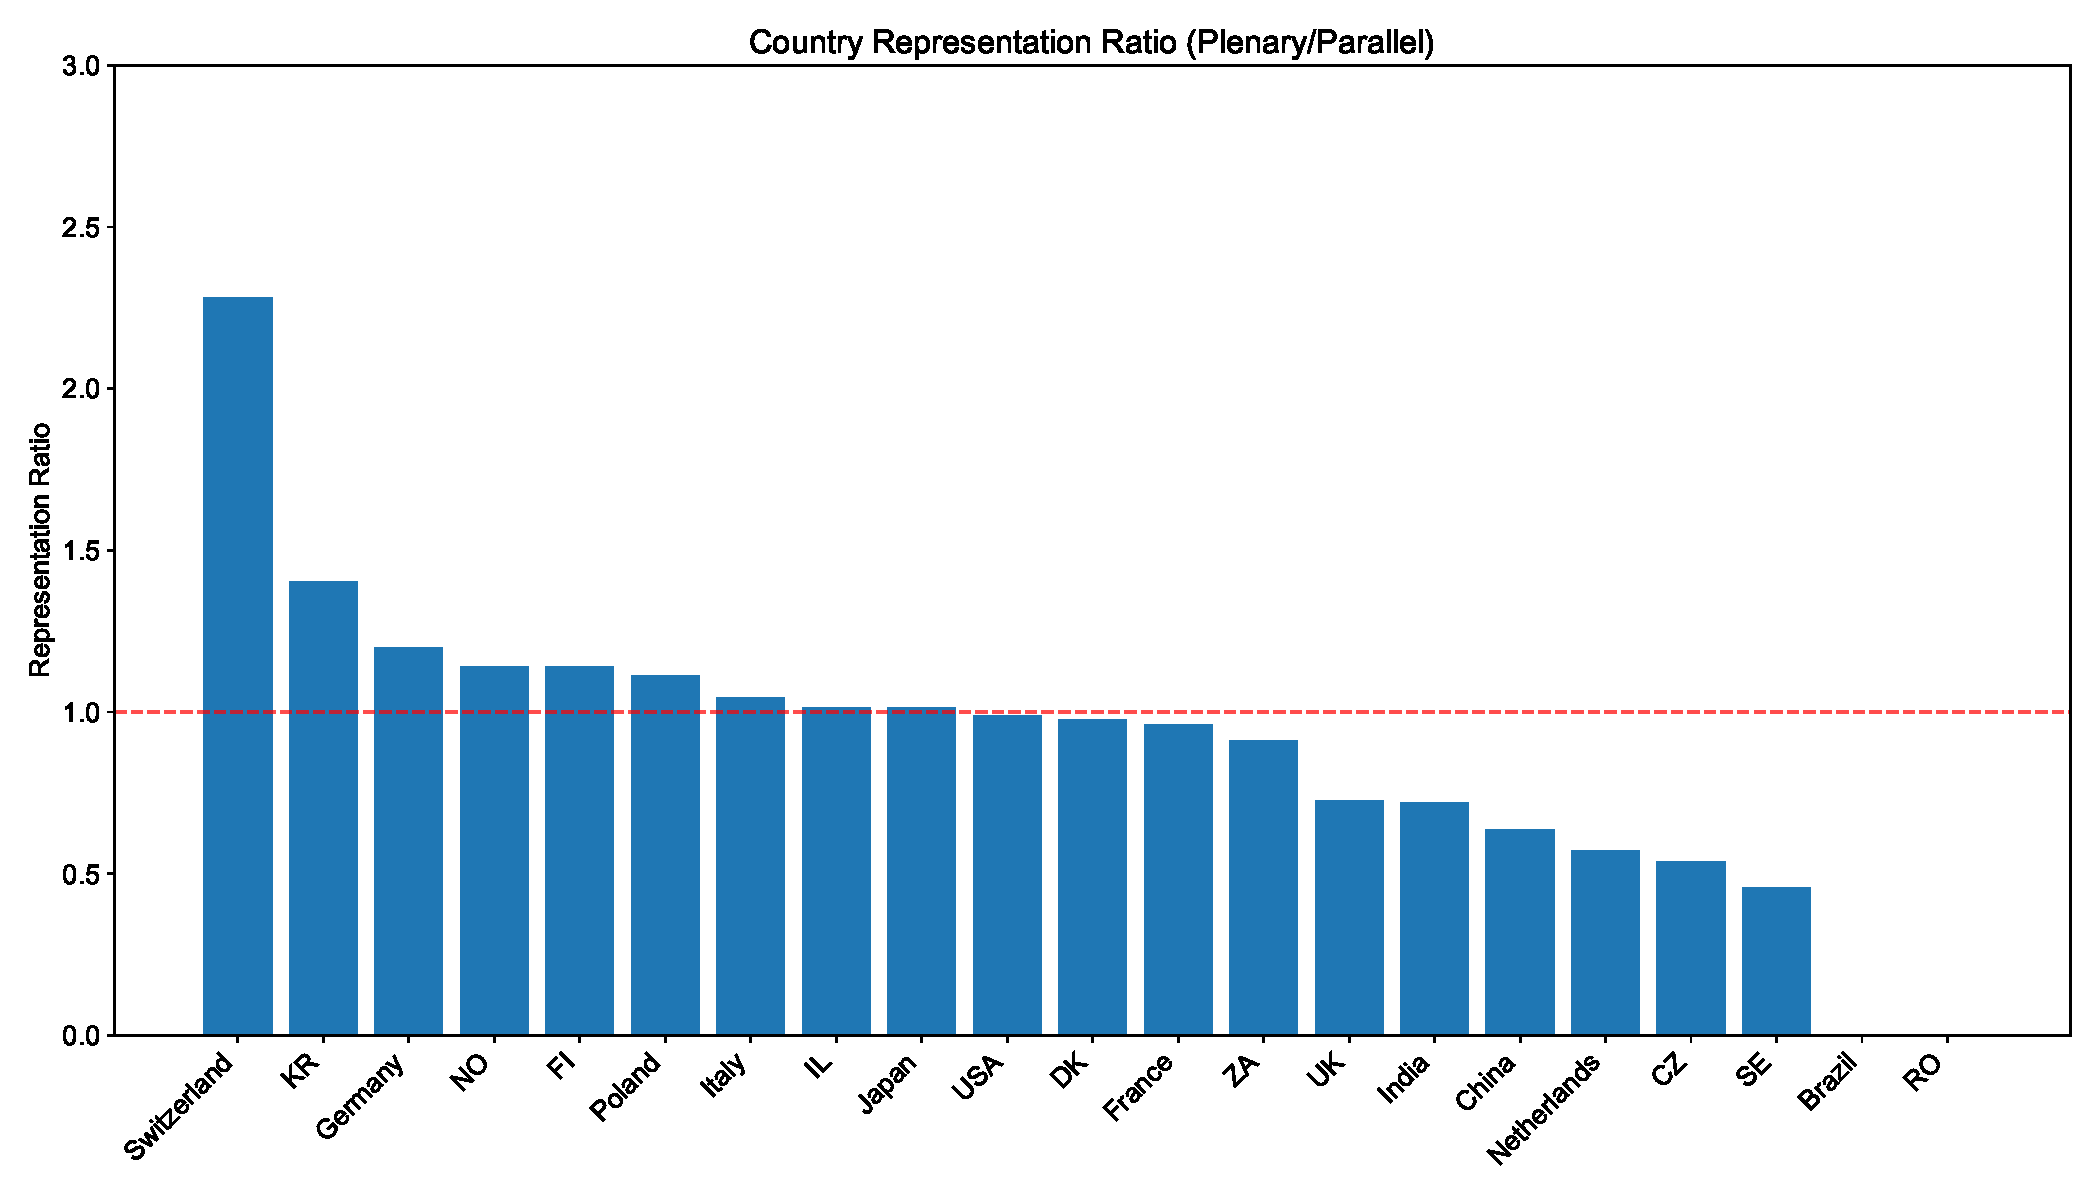
\includegraphics[width=\textwidth]{figures/representation_ratio.pdf}
\caption{Representation ratio between plenary and parallel talks by country. This chart compares each country's share of high-visibility plenary talks to their share of parallel sessions, with values above 1.0 indicating overrepresentation and values below 1.0 indicating underrepresentation. With improved data completeness from our enhanced affiliation resolution system, these representation metrics more accurately reflect actual participation patterns and structural imbalances in speaking opportunities.}
\label{fig:representation_ratio}
\end{figure}

\begin{figure}[H]
\centering
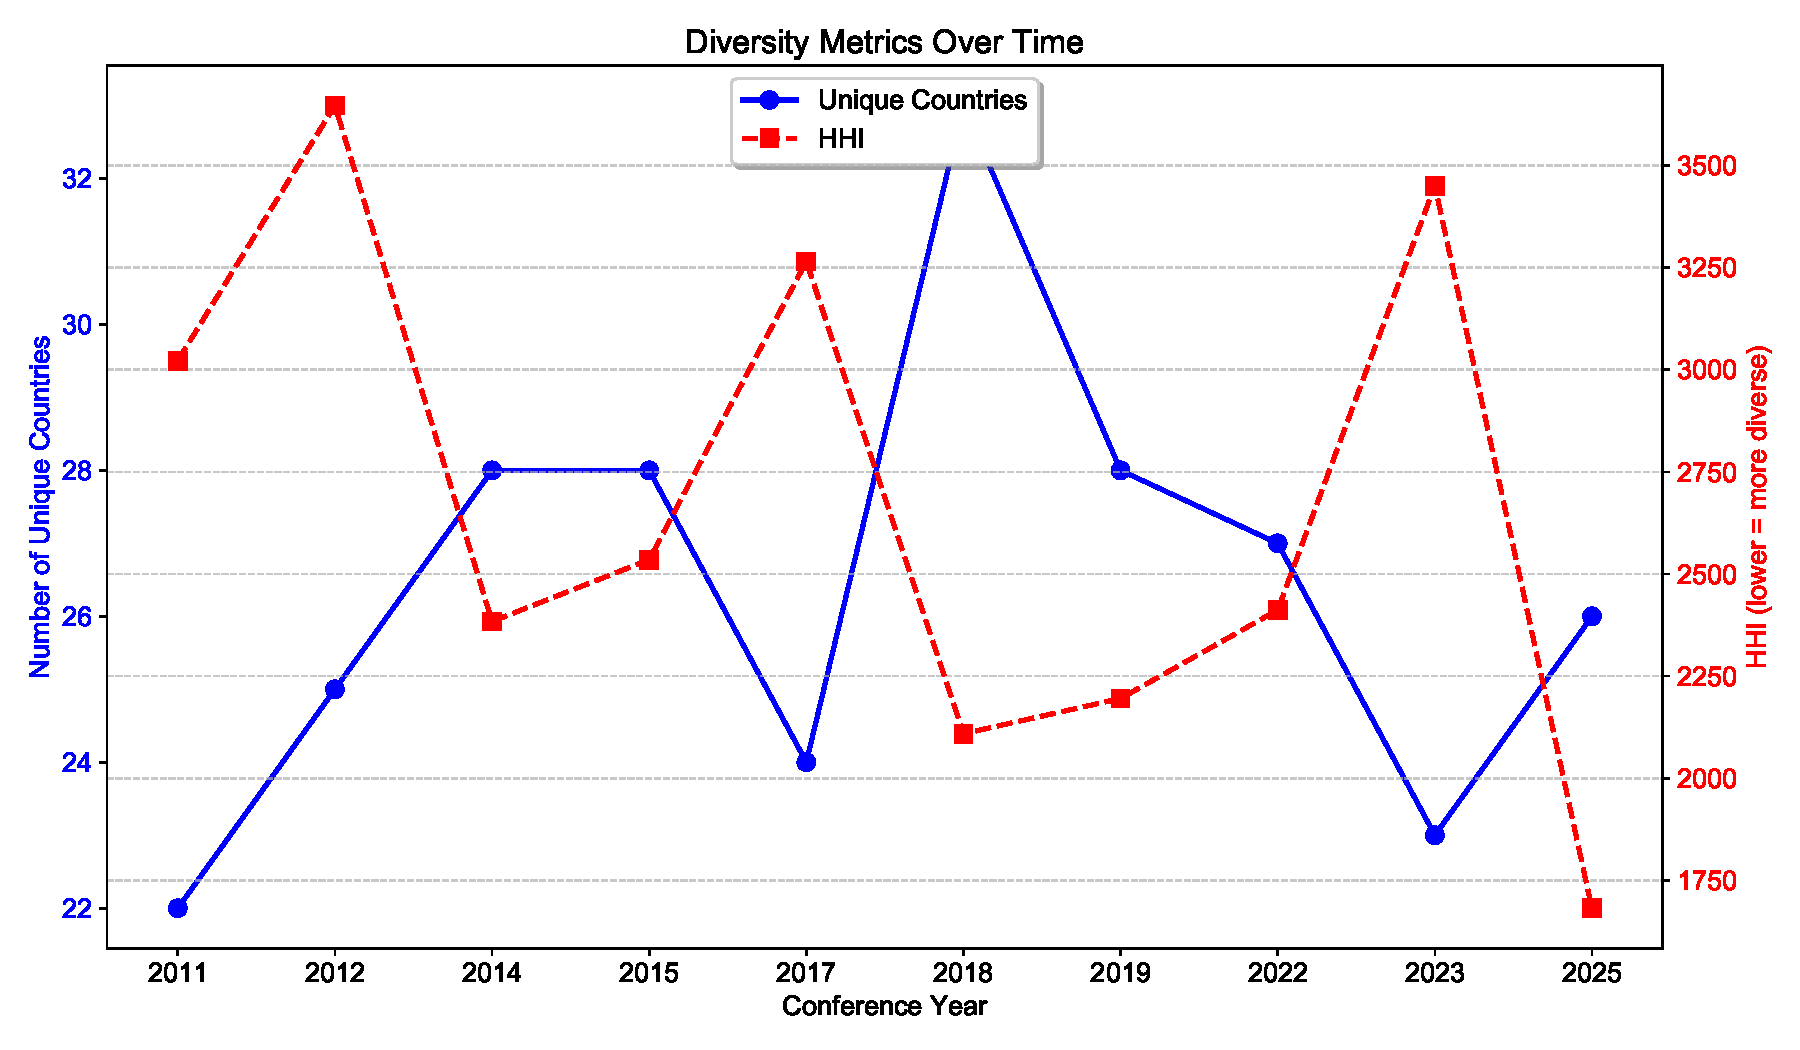
\includegraphics[width=\textwidth]{figures/diversity_metrics.pdf}
\caption{Evolution of diversity metrics over time. The top panel shows the number of unique countries represented at each conference, while the bottom panel displays the Herfindahl-Hirschman Index (HHI), a measure of concentration where lower values indicate more diverse representation. Our enhanced country resolution methodology allows for more accurate tracking of these diversity metrics by minimizing the number of contributions with unknown origins.}
\label{fig:diversity_metrics}
\end{figure}

\section{Discussion}

\subsection{Diversity and Representation}

Our analysis of geographical and institutional representation at Quark Matter conferences reveals persistent patterns that merit careful consideration. The concentration of presentations, particularly high-visibility plenary talks, among a small group of countries and institutions suggests structural imbalances in how research visibility is distributed in the field.

While some degree of concentration is expected given differences in community size, research infrastructure, and historical development of the field in different regions, the persistence of these patterns across multiple conference cycles raises questions about the mechanisms of speaker selection and the potential for implicit biases in these processes.

Our improved data resolution methodology offers greater confidence in these findings by substantially reducing missing or unknown affiliations. The enhanced completeness of country and institution data ensures that our observations about geographical representation are based on more robust evidence rather than potentially skewed by systematic gaps in the dataset. This is particularly important for accurately assessing the representation of smaller countries and institutions, where even a small number of misclassified or missing entries could significantly impact the apparent level of participation.

The data suggests several potential approaches for conference organizers interested in enhancing diversity of representation:

\begin{itemize}
    \item Implementing transparent selection criteria that explicitly value geographical and institutional diversity alongside scientific excellence
    \item Developing mentoring programs or speaking opportunities specifically designed to highlight researchers from underrepresented institutions and countries
    \item Rotating conference locations more systematically to encourage broader participation and reduce travel barriers
    \item Collecting and monitoring demographic data on conference participation to track progress over time
    \item Implementing regional quotas or targets that ensure representation from a broader range of countries while maintaining scientific excellence
    \item Creating mentoring or speaking opportunity programs specifically for researchers from emerging countries in the field
\end{itemize}

Importantly, our findings suggest that addressing these imbalances may require attention not just to country-level representation but to institutional diversity within countries, as the institutional concentration appears even stronger than geographical concentration.

\subsection{Evolution of Research Focus}

The keyword analysis provides a fascinating window into how the scientific focus of the heavy-ion physics community has evolved over the past decade. Several key patterns emerge:

\begin{itemize}
    \item A shift from facility-focused research (emphasized by accelerator and detector keywords) toward more phenomenon-focused investigations
    \item The rise and fall of certain research themes, reflecting the community's response to new discoveries and theoretical developments
    \item Increasing specialization and technical sophistication, as indicated by the growing specificity of keywords in later conferences
    \item The emergence of new research directions, particularly investigations of collectivity in small systems and the application of machine learning techniques
\end{itemize}

These trends reflect a field in transition, moving from an early phase focused on establishing the basic properties of the quark-gluon plasma toward more detailed investigations of specific phenomena and increasingly precise measurements. The keyword dynamics also highlight the responsiveness of the field to surprising experimental results, such as the observation of collective behavior in small collision systems.

\subsection{Implications for Conference Organization}

Based on our findings, several recommendations emerge for future Quark Matter conference planning:

\begin{itemize}
    \item Implementation of more transparent and explicitly diversity-conscious selection processes for talks, particularly plenary presentations
    \item Consideration of mechanisms to provide speaking opportunities for researchers from underrepresented countries and institutions
    \item Balancing representation of established research directions with emerging topics to ensure the conference remains at the cutting edge
    \item Improving data collection on speaker demographics to better track progress on diversity goals
    \item Developing structures to highlight work from smaller or newer research groups, potentially through dedicated sessions or presentation formats
    \item Implementing regional quotas or targets that ensure representation from a broader range of countries while maintaining scientific excellence
    \item Creating mentoring or speaking opportunity programs specifically for researchers from emerging countries in the field
\end{itemize}

These measures would help ensure that Quark Matter conferences continue to serve as inclusive forums that represent the full breadth of the international heavy-ion physics community.

\section{Conclusion}

This historical analysis of Quark Matter conferences provides valuable insights into the evolution of heavy-ion physics as reflected in its premier conference series. By quantifying patterns of participation, geographical distribution, and research focus, we have established a factual basis for discussions about how these conferences might better serve the scientific community.

Our findings reveal both strengths and areas for improvement in the current structure of these conferences. The keyword analysis demonstrates a vibrant field addressing an evolving set of scientific questions with increasing sophistication. At the same time, the geographical and institutional analyses highlight persistent patterns of concentration that may not fully reflect the global nature of the field.

As Quark Matter conferences continue to evolve, regular analysis of participation patterns can provide valuable feedback to organizers and the community as a whole. By making these patterns visible, we hope to contribute to ongoing discussions about how to ensure these important scientific gatherings reflect the diversity and dynamism of heavy-ion physics research worldwide.

\section{Acknowledgments}

We thank the organizers of Quark Matter conferences for making the presentation data publicly available through Indico, enabling this analysis.

\bibliographystyle{unsrt}
\begin{thebibliography}{9}
\bibitem{indico} 
CERN. ``Indico - Event Management System.'' 
\texttt{https://indico.cern.ch/}

\bibitem{QM2011}
Quark Matter 2011 Conference Proceedings,
\texttt{https://indico.cern.ch/event/30248/}

% Additional references would be added here
\end{thebibliography}

\end{document}